%% Chapter 9 — 모델 서빙 프레임워크
\setcounter{chapter}{8}
\chapter{모델 서빙 프레임워크}
\chaptersubtitle{모델 서버의 구조, 배치 처리의 절충 관계, 대표 프레임워크 네 가지 — 그리고 모두를 정직하게 만드는 Locust}

\begin{calloutbox}{tbbblue}{tbbbluefill}
{\normalsize\bfseries\color{tbbblue}학습 목표}\par\vspace{3pt}
\begin{tbbitemize}
  \item Locust 표 하나와 \code{nvidia-smi} 줄 하나를 보고 직접 만든 모델 서버가 GPU 성능의 일부에서 정체되는 이유를 진단하고, 간격을 메우는 세 가지 엔지니어링인 배치 처리, 파이프라이닝, 동시성을 말한다.
  \item 프로덕션 모델 서버의 \textbf{여섯 기관}인 프런트엔드, 대기열+배처, 인스턴스, 모델 관리, 관측 가능성, 상태 확인/수명 주기를 그리고 각각을 필요하게 만든 실패와 연결한다.
  \item \textbf{동적 배치 처리}의 두 설정값, 지연 시간–처리량 절충 관계, 상한을 정하는 VRAM 경계를 구성하고 논리적으로 분석하며, 벤치마크 차트가 아니라 \textit{SLO를 기준으로} 배치 상한을 고른다.
  \item 같은 여섯 기관을 바라보는 네 가지 철학으로 \textbf{Triton, TorchServe, BentoML, Ray Serve}를 비교하고 네 질문 체크리스트로 선택하며, vLLM과 KServe가 경쟁자가 아니라 이웃인 이유를 이해한다.
  \item 개방 루프 페이싱, 유효 처리량, 리틀의 법칙 감사를 포함한 정직한 Locust 스윕을 실행하고 제안서에 필요한 단 하나의 숫자인 SLO에서 레플리카당 req/s를 추출한다.
  \item 의도적으로 \textbf{재시도 폭풍}을 재현하고 증폭된 도착 요청, 붕괴한 유효 처리량, 복구 불가라는 파형을 알아보며, 이를 막는 재시도 예산 규칙을 설명한다.
\end{tbbitemize}
\end{calloutbox}

\vspace{3.5pt}

\begin{calloutbox}{tbbteal}{tbbtealfill}
{\normalsize\bfseries\color{tbbteal}핵심 용어}\par\vspace{3pt}
모델 서버 · 서빙 프레임워크 · 동적 배치 처리 · 최대 배치 크기 · 최대 대기열 지연 · 인스턴스 그룹 · 모델 저장소 · 핸들러 · 앙상블 · 유효 처리량 · 개방 루프 페이싱(고정 처리량) · 재시도 폭풍 · 부하 차단 · Triton · TorchServe · BentoML · Ray Serve · 이웃: vLLM · KServe
\end{calloutbox}

\vspace{3.5pt}

\begin{calloutbox}{tbblightgray}{tbbboxfill}
{\normalsize\bfseries\color{tbbink}장 구성}\par\vspace{3pt}
\textbf{9.1} 정중한 서버와 6개월 로드맵    \textbf{9.2} 모델 서버의 구조: 여섯 기관    \textbf{9.3} 동적 배치 처리: 두 설정값과 하나의 절충 관계    \textbf{9.4} 대표 프레임워크 네 가지와 선택 방법    \textbf{9.5} Locust: 중요한 숫자를 제대로 측정하기    \textbf{9.6} 실습: 서빙하고, 스윕하고, 의도적으로 폭풍 만들기 — 이어서 요약, 연습문제, 더 읽을거리.
\end{calloutbox}

\section{정중한 서버와 6개월 로드맵}

4주 차 FastAPI 서버는 지금까지 제 몫을 다했다. 컨테이너를 가르치고(제4장), 스케줄링되고(제5장), 스토어에서 가중치를 가져오는 법을 배우고(제6장), 제안서의 첫 벤치마크 기준이 되었다(제7장). 이번 주에는 프로덕션 트래픽의 첫 질문인 \textit{얼마나 많이 처리할 수 있는가?}를 마주한다. 정직하게 답하려면 사례가 필요하다. 실습에서 사용한 이미지 분류기를 강의 T4의 레플리카 하나에서 실행하고, Locust에게 사용자 60명이 낼 수 있는 만큼 강하게 밀도록 한다.

\subsection*{사례 A: 정체 구간}

\begin{terminalbox}
\begin{Verbatim}[breaklines=true,breakanywhere=true,fontsize=\small,formatcom=\color{tbbtermfg},codes=\tbbcodeactive]
$ locust -f locustfile.py --headless -u 60 -r 10 --run-time 5m \
         --host http://clf.demo.internal
 Type  Name         # reqs  # fails |  Avg    p50    p99  | req/s
 POST  /classify    3,529   0(0.0%) | 4,913  4,800  8,102 | 11.8
# sixty users pushing as hard as they can: 11.8 req/s. the ceiling.
$ kubectl exec deploy/clf -- nvidia-smi \
         --query-gpu=utilization.gpu --format=csv,noheader
7 %                        # the "AI server" is 93% idle...
$ kubectl top pod -l app=clf
NAME         CPU(cores)   MEMORY(bytes)
clf-6d9f4    996m         2913Mi
# ...while ONE cpu core runs flat out. there is your server.
\end{Verbatim}
\end{terminalbox}
\figcaption{사례 9-A  정체 구간. 기꺼이 요청을 보내는 사용자 60명, 11.8 req/s, 5초 대기인데 GPU는 7\%에서 놀고 CPU 코어 하나만 포화한다. 고장 난 것은 없고 모두가 지나치게 정중할 뿐이다.}

제7장의 도구로 부검해 보자. 사례의 모든 숫자는 한 가지 설계 사실에 의해 산술적으로 강제된다. \textbf{서버가 Python 스레드 하나에서 한 번에 요청 하나를 처음부터 끝까지 처리한다.} 요청마다 CPU에서 이미지 디코딩과 크기 조정에 \textasciitilde{}60 ms, 실제 GPU 추론에 \textasciitilde{}8 ms, 답 직렬화에 \textasciitilde{}15 ms를 쓴다. 직렬 작업이 \textasciitilde{}83 ms이므로 상한은 1 ÷ 0.083 ≈ \textbf{12 req/s}다. 사례 1-A의 계산이 세 번째 등장했다. 리틀의 법칙도 자백에 서명한다. 11.8 req/s로 동작하는 폐쇄 루프 사용자 60명은 각각 W = 60 ÷ 11.8 ≈ \textbf{5.1 s}를 기다려야 한다. 평균 열을 소수점까지 예측했다. GPU는 매초 11.8 × 8 ms ≈ \textbf{9\%}만 바쁘며 \code{nvidia-smi}가 이를 보여 준다. 고정된 코어 하나는 초당 11.8번 도착하는 60 ms 전처리를 담당한다. 제1장은 GPU를 수천 명의 작업자 부대라고 불렀다. 이 서버는 부대에 티스푼으로 일을 먹이면서 부대 가격을 낸다(그림 9-1).

\begin{tbbfigure}
  \adjustbox{max width=0.94\linewidth,max totalheight=0.46\textheight}{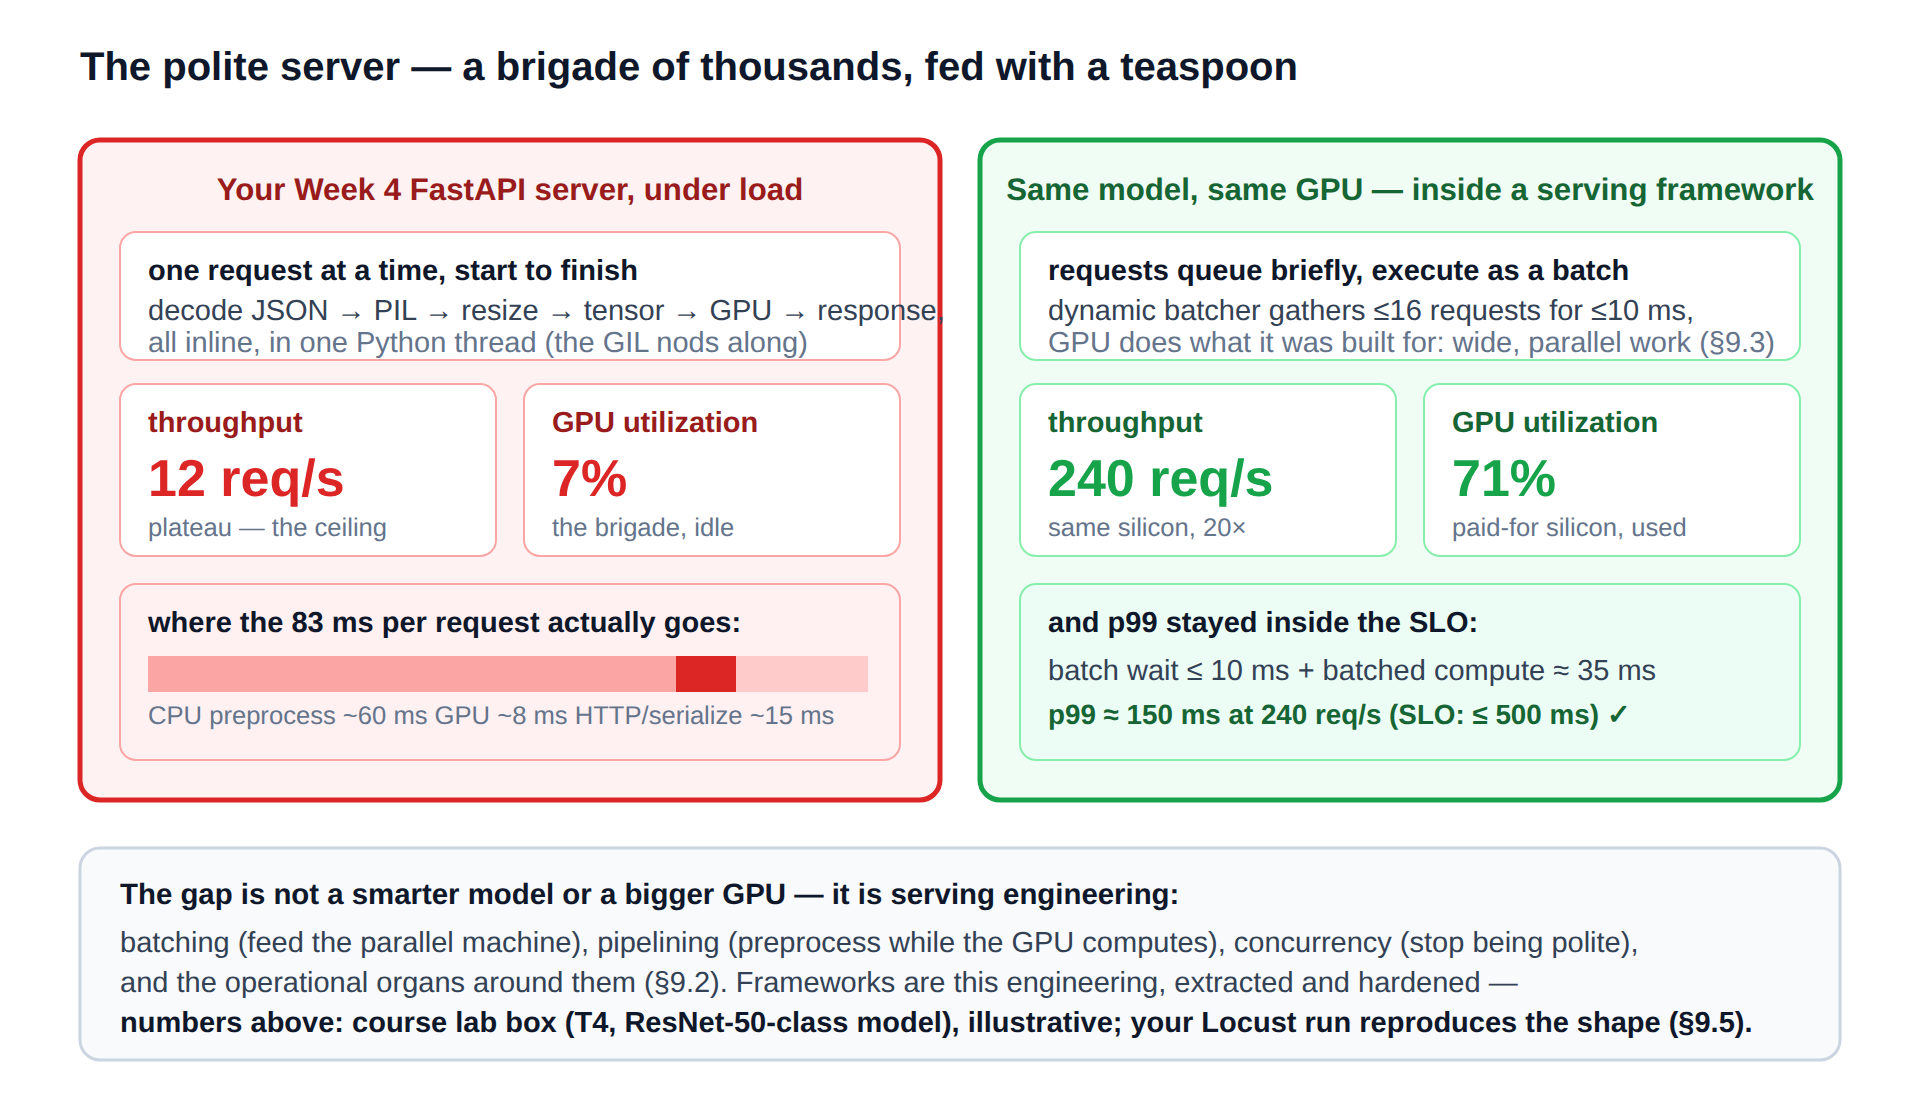
\includegraphics{figures/fig9-1_teaspoon.png}}\\[3pt]
  \figcaption{그림 9-1  숫자로 본 티스푼. 같은 모델과 같은 T4에서 정중한 서버는 12 req/s와 GPU 7\%에서 정체하고, 서빙 프레임워크의 배치 처리와 파이프라이닝은 SLO 안에서 240 req/s와 71\%에 도달한다.}
\end{tbbfigure}

세 가지 엔지니어링으로 간격을 메울 수 있으며 더 똑똑한 모델은 하나도 없다. \textbf{배치 처리}는 요청을 잠깐 모아 한 번의 넓은 GPU 실행으로 처리한다. 이 장의 주인공인 §9.3에서 다룬다. \textbf{파이프라이닝}은 번갈아 처리하지 않고 GPU가 배치 N을 계산하는 \textit{동안} CPU가 요청 N+1을 전처리한다. \textbf{동시성}은 여러 실행 스트림을 사용해 머신이 요청 하나의 왕복을 정중하게 기다리지 않게 한다. 세 가지 모두 직접 구현할 수 있다. 그렇다면 이 장의 실제 질문은 \textit{직접 해야 하는가?}다.

\subsection*{사례 B: 6개월 로드맵 또는 수렴 진화}

"그렇다"고 답한 모든 팀에 일어나는 일을 보자. 아래 git 로그는 여러 사례를 합쳤지만 ML 인프라 엔지니어에게 검토해 달라고 하면 알아보고 몸서리칠 것이다. 대부분의 커밋을 직접 작성해 보았기 때문이다.

\begin{terminalbox}
\begin{Verbatim}[breaklines=true,breakanywhere=true,fontsize=\small,formatcom=\color{tbbtermfg},codes=\tbbcodeactive]
$ git log --oneline --reverse -- serving/   # one team, eight months
a3f1e02  feat: flask server for resnet, MVP           (day 1)
9c02b11  fix: load model ONCE at startup not per req   (day 3. oops.)
5e77a4d  feat: /healthz + /ready (k8s kept killing us) (week 2)
b8d0c9e  feat: worker pool + request queue             (week 5)
1f6602a  feat: micro-batching, 10ms window (GPU util!) (week 7)
77ab3f0  feat: /metrics for prometheus                 (week 9)
c90d1f4  feat: serve model v2 alongside v1, split      (week 14)
e01b772  fix: drain in-flight reqs on SIGTERM          (week 15. outage.)
4d9a8c3  feat: config-driven model loading from s3     (week 19)
f33c6b8  docs: "how our serving works" (34 pages)      (week 23)
# congratulations: you have rebuilt 2016's TF-Serving.
# minus the tests, the docs, and the other users.
\end{Verbatim}
\end{terminalbox}
\figcaption{사례 9-B  수렴 진화. 직접 만든 서버를 유지하는 모든 팀은 정확히 이 커밋 이력을 걷는다. 각 커밋은 프로덕션이 어김없이 제공하는 실패에 답하기 때문이다. 도착점에는 서빙 프레임워크라는 이름이 있다.}

로그를 생물학처럼 읽어 보자. 추측으로 만든 것은 아무것도 없다. 각 커밋은 특정 실패가 남긴 흉터 조직이다. 3일째의 요청별 재로딩, 2주째의 활성 상태 검사에 따른 종료, 15주째 배포 중 누락된 요청이 있으며 제5장과 제3장이 뒤의 두 가지를 예측했다. 프로덕션은 어디서나 같은 선택 압력을 가하므로 팀마다 \textit{순서}도 거의 다르지 않다. 서로 다른 조직이 내부 서빙 스택을 오픈 소스로 공개했을 때 결과물에 모두 같은 기관이 있었던 이유다. 이 실패를 다른 조직보다 몇 년 먼저 겪은 Google의 \textbf{TensorFlow Serving}(2016)이 먼저 나왔고, 이어 NVIDIA의 TensorRT Inference Server(2018, 2020년 \textbf{Triton}으로 이름 변경), \textbf{TorchServe}(2020), Python 우선 물결인 \textbf{BentoML}과 \textbf{Ray Serve}가 등장했다. 서빙 프레임워크는 제품 범주라기보다 화석 기록이다. 모두가 보낸 6개월을 추출해 단단하게 만들고 다른 누군가가 유지한다. 따라서 이 장이 답할 수 있게 하는 엔지니어링 질문은 "만들 수 있는가?"가 아니다. 만들 수 있고 사례 9-B가 일정표다. 질문은 \textbf{"어느 실패부터 다시 발견하기를 멈출 것인가?"}다.

\subsection*{이 장의 어휘}

\begin{tbbtablewrap}
  \begin{tabular}{@{}>{\raggedright\arraybackslash}m{\dimexpr 0.2660\tbltextwidth-2\tabcolsep\relax} >{\raggedright\arraybackslash}m{\dimexpr 0.7340\tbltextwidth-2\tabcolsep\relax}@{}}
  \arrayrulecolor{tbbnavy}\specialrule{1pt}{0pt}{0pt}
  \rowcolor{tbbtablehead}{\centering \bfseries\color{tbbnavy}용어} & {\centering \bfseries\color{tbbnavy}의미} \\
  \arrayrulecolor{tbbnavy}\specialrule{0.7pt}{0pt}{2pt}
  {\textbf{모델 서버}} & {모델 아티팩트(§7.6)를 로딩하고 추론 요청에 응답하는 프로세스. 사례 9-A의 피고이자 §9.2의 환자다.} \\
  \arrayrulecolor{tbbtableborder}\hline
  {\textbf{서빙 프레임워크}} & {모델 서버의 여섯 기관(§9.2)을 유지 관리되는 형태로 구현한 것. Triton, TorchServe, BentoML, Ray Serve가 있다.} \\
  \arrayrulecolor{tbbtableborder}\hline
  {\textbf{동적 배치 처리}} & {동시 요청을 서버에서 한 번의 GPU 실행으로 모으는 방식. 최대 배치 크기와 최대 대기열 지연으로 제한한다(§9.3).} \\
  \arrayrulecolor{tbbtableborder}\hline
  {\textbf{인스턴스 그룹}} & {GPU 하나 또는 여러 GPU에서 실행되는 모델 복사본 N개. 계산과 전처리/후처리를 겹치게 한다. Triton의 명칭이며 모든 프레임워크에 대응 요소가 있다.} \\
  \arrayrulecolor{tbbtableborder}\hline
  {\textbf{모델 저장소}} & {프레임워크가 지켜보는 디렉터리 트리. 로컬 또는 제6장의 스토어를 직접 쓰는 s3://이며 모델 × 버전 × 설정을 런타임에 로딩할 수 있다.} \\
  \arrayrulecolor{tbbtableborder}\hline
  {\textbf{핸들러}} & {프레임워크가 모델 앞뒤에서 실행하는 사용자 코드(전처리/후처리). TorchServe의 용어이며 BentoML과 Ray는 일반 Python으로 표현한다.} \\
  \arrayrulecolor{tbbtableborder}\hline
  {\textbf{앙상블/그래프}} & {클라이언트 왕복 없이 실행하는 모델과 단계의 서버 측 파이프라인(전처리 → 모델 → 후처리).} \\
  \arrayrulecolor{tbbtableborder}\hline
  {\textbf{유효 처리량}} & {SLO 안에서 성공한 요청만 세는 처리량. 시간 초과와 오류가 표를 채울 때 중요한 숫자다(§9.5).} \\
  \arrayrulecolor{tbbtableborder}\hline
  {\textbf{개방 루프 페이싱}} & {응답과 무관하게 고정 도착률로 부하를 생성하는 방식(Locust의 constant\_throughput). §7.3의 정직성 요구를 구현한다.} \\
  \arrayrulecolor{tbbtableborder}\hline
  {\textbf{재시도 폭풍}} & {이미 포화한 서버에서 클라이언트 재시도가 도착 요청을 늘려 스스로 유지되는 과부하다. 유효 처리량이 붕괴하고 복구되지 않는다(§9.5).} \\
  \arrayrulecolor{tbbnavy}\specialrule{1pt}{2pt}{0pt}
  \end{tabular}\par
  \figcaption{표 9-1  이 장에서 사용할 어휘}
\end{tbbtablewrap}

\begin{calloutbox}{tbbpurple}{tbbpurplefill}
{\normalsize\bfseries\color{tbbpurple}생각해 보기}\par\vspace{3pt}
\begin{tbbitemize}
  \item 사례 9-A의 내부 일관성을 직접 검증하자. 서비스 시간 83 ms와 폐쇄 루프 사용자 60명으로 상한, 평균 대기 시간, GPU 사용률을 도출한다. 각각 제7장의 두 도구 가운데 무엇을 사용했는가? 이 장에서 시험 문제를 낸다면 바로 이것이다.
  \item 사례 9-B의 각 커밋을 자라나게 한 §9.2의 기관과 연결하자. 일부는 두 기관에 해당한다. 어떤 커밋 두 개가 기능이 아니라 \textit{장애}였으며 이 책의 어느 장이 예측했는가?
  \item 사례 9-B의 팀은 \textasciitilde{}8개월을 썼다. 엔지니어 두 명의 비용을 "2주 동안 Triton 학습"과 비교한 뒤, 그래도 직접 만드는 것이 옳은 상황을 말하자. 극단적인 사용자 정의 프로토콜, 특이한 하드웨어처럼 실제 사례가 있지만 경력 과시용 개발은 포함되지 않는다.
\end{tbbitemize}
\end{calloutbox}

\section{모델 서버의 구조: 여섯 기관}

제품을 비교하기 전에 기본 구조부터 익히자. 8개월 동안 직접 만든 서버든 바로 설치한 프레임워크든 진지한 모델 서버는 모두 같은 여섯 기관으로 수렴한다(그림 9-2). 각 기관이 프로덕션이 어김없이 제공하는 실패 하나에 답하기 때문이다. 프레임워크의 철학은 다르지만(§9.4) 기관은 같다. 각 기관이 존재하는 이유를 처음 만난 장과 연결하며 한 번 살펴보자.

\begin{tbbfigure}
  \adjustbox{max width=0.94\linewidth,max totalheight=0.46\textheight}{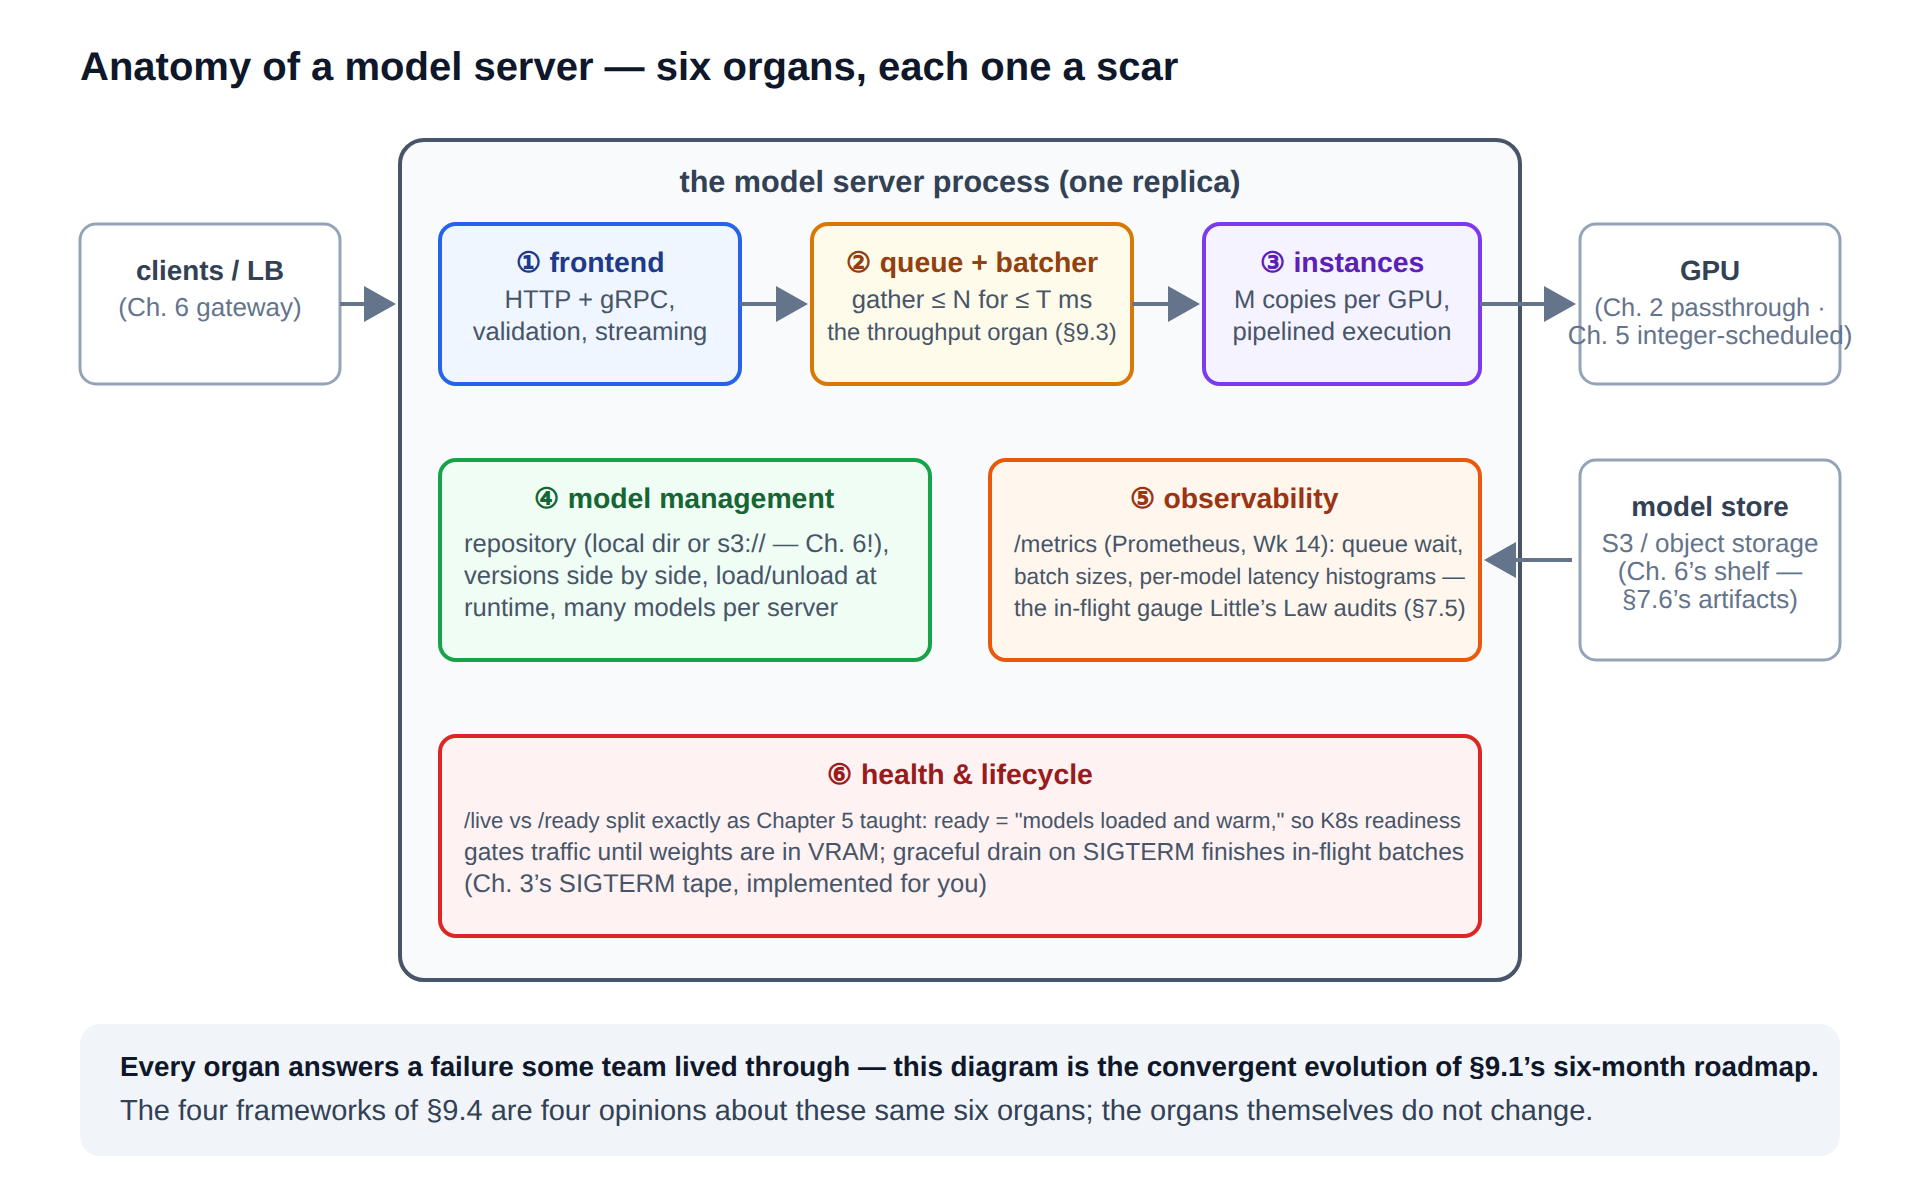
\includegraphics{figures/fig9-2_anatomy.png}}\\[3pt]
  \figcaption{그림 9-2  모델 서버의 여섯 기관. 각 상자는 특정 프로덕션 실패에 답하고, §9.4의 프레임워크 네 가지는 같은 구조를 바라보는 네 가지 견해다.}
\end{tbbfigure}

\subsection*{① 프런트엔드: 프로토콜, 검증, 출입구 정책}

프런트엔드는 제6장 게이트웨이의 공용어인 HTTP를 사용하고, 진지한 배포에서는 초당 요청량이 많은 내부 호출자를 위해 \textbf{gRPC}도 사용한다. gRPC의 이점은 구체적이다. 이미지나 텐서는 base64로 부풀린 JSON(+33\% 바이트와 두 번의 디코딩 단계)이 아니라 압축된 이진 프레임의 원시 바이트로 이동하고, 하나의 다중화 연결이 계속 반복되는 HTTP 핸드셰이크를 대신한다. 작은 텐서를 1,000 req/s로 보낼 때 직렬화 비용은 지연 시간 예산에서 눈에 보이는 몫이지만 큰 이미지를 10 req/s로 보낼 때는 차이를 알아채기 어렵다. 프런트엔드는 출입구 정책도 강제한다. \textbf{GPU 전에 검증}해야 한다. 잘못된 이미지는 배치 자리를 소비한 뒤 CUDA 커널 깊은 곳에서 500 오류로 죽는 대신 몇 마이크로초 안에 출입구에서 400 오류로 거부되어야 한다. 방식이 요구하면 스트리밍 응답도 구현한다(§7.2). 그래서 "프록시 체인이 서버 전송 이벤트를 버퍼링 없이 전달할 수 있는가?"가 제6장의 질문이었다.

\subsection*{② ③ 대기열, 배처, 인스턴스: 성능 기관}

\textbf{대기열과 배처}에는 이 장의 경제학이 담겨 있다. §9.3 전체에서 다루므로 여기서는 위치만 중요하다. 프런트엔드 뒤의 서버 \textit{내부}에 있어 요청을 검사하고 모델과 형태별로 묶으며 의도적으로 스케줄링할 수 있다. 4주 차 서버에 가장 부족했던 부분이다. 그 서버의 "대기열"은 우연히 TCP 연결 수락 대기 목록에 들어간 것이 전부였고 보이지 않으며 측정하거나 관리할 수 없었다. §7.5의 리틀 감사가 계속 찾아내던 숨은 대기열이다. \textbf{인스턴스}는 세 번째 성능 기관이다. 프레임워크는 GPU 하나에서 모델의 \textit{실행 가능한 복사본 M개}를 돌린다. 복사본 하나가 배치를 계산하는 동안 두 번째 복사본의 입력을 디코딩해 장치로 복사한다. 사례 9-A의 번갈아 처리하는 낭비를 고치는 파이프라이닝이다. M은 실제 설정값이다. 2는 계산과 데이터 전송을 겹쳐 흔히 공짜 성능을 주지만, 8은 복사본이 하나의 SM 집합과 PCIe 버스를 공유하므로 대부분 경합만 산다. 제5장의 나눌 수 없는 정수 GPU를 내부에서 체감하는 셈이다. §9.5 스윕에 실행 하나를 더하면 경험적으로 조정할 수 있다.

\subsection*{④ 모델 관리: 지켜보는 선반}

직접 만든 서버가 가장 늦게 키우고 프레임워크는 가장 먼저 제공하는 기관이 모델 관리다. 서버가 \textit{지켜보는} 모델 × 버전 디렉터리 트리인 \textbf{모델 저장소}를 두고 로딩과 언로딩을 배포가 아니라 API 호출로 수행한다. 여기서 강의의 두 흐름이 맞물린다. 첫째, 저장소는 객체 스토어의 접두사인 \code{s3:/\allowbreak /\allowbreak models/\allowbreak prod/\allowbreak } 자체일 수 있다. 제6장의 선반을 그대로 사용한다. Triton은 이를 폴링하고 예상한 병렬 범위 GET으로 새 버전을 가져오며 코드에 넣은 키 대신 IRSA로 인증한다. 둘째, 버전을 나란히 두면 13주 차 배포가 영웅적인 일이 아니라 기계적인 일이 된다. v7과 v6가 모두 로딩되어 예열된 상태이고, 트래픽 분할은 상류 시스템이 결정하며, 롤백은 레이블을 다시 가리키는 일이다. 재배포가 아니라 몇 초면 된다. 하나의 서버 프로세스가 모델별 설정과 메트릭을 갖춘 \textit{여러} 모델을 호스팅하는 방식은 롱테일 플릿의 경제적 답이기도 하다. 각각 사용률 3\%인 작은 모델 40개에 GPU 40개를 줄 이유는 없다. 제1장의 유휴 부대 계산을 플릿 규모로 적용한 것이다.

\subsection*{⑤ 관측 가능성: 제7장이 요구한 게이지}

관측 가능성 기관은 Prometheus 형식의 \code{/\allowbreak metrics} 엔드포인트다. 이를 읽는 일은 제7장 시험을 축소해 놓은 것과 같다.

\begin{terminalbox}
\begin{Verbatim}[breaklines=true,breakanywhere=true,fontsize=\small,formatcom=\color{tbbtermfg},codes=\tbbcodeactive]
$ curl -s localhost:8002/metrics | grep -E "queue|batch|count" | head -12
# latency as HISTOGRAM BUCKETS - rule 4: aggregate buckets, never p99s
nv_inference_request_duration_us_bucket{model="resnet50",le="50000"} 9871
nv_inference_request_duration_us_bucket{model="resnet50",le="100000"} 11209
# where time is spent: queue vs compute, separately measured
nv_inference_queue_duration_us{model="resnet50"}    8.31e+08
nv_inference_compute_infer_duration_us{...}         2.94e+09
# the in-flight facts for the Little audit (§7.5):
nv_inference_pending_request_count{model="resnet50"} 19
# and how well batching is working - the histogram that explains
# "throughput fell when traffic went trickle":
nv_inference_batch_size_bucket{le="8"} 4102   {le="16"} 9877  ...
\end{Verbatim}
\end{terminalbox}
\figcaption{터미널 기록 9-1  주석을 단 모델 서버의 /metrics. 지연 시간은 히스토그램 버킷으로 전송되고(백분위수를 평균할 수 없다는 제7장 규칙 ④), 대기 시간과 계산 시간은 분리되며, 처리 중 요청 게이지는 리틀 감사에 쓰이고, 배치 크기 히스토그램은 §9.3의 절충 거래가 실제로 이루어지는지 알려 준다.}

두 가지 세부사항을 강조할 가치가 있다. 대기 시간과 계산 시간은 \textit{별도} 카운터로 온다. 그래서 "지연 시간이 늘었다"를 쿼리 하나로 "대기가 늘었다"(용량/변곡점 문제, §7.5)와 "계산이 늘었다"(모델/하드웨어 문제)로 나눌 수 있다. 14주 차 대시보드 설계의 절반을 대신 해 준 셈이다. 배치 크기 분포는 배처의 정직성 계기다. 트래픽 구성이 바뀌면 배치 처리 효과가 조용히 달라지고 이 히스토그램만 이를 목격한다.

\subsection*{⑥ 상태 확인과 수명 주기: 과거 장애의 재발을 막는 기관}

상태 확인과 수명 주기는 제5장의 프로브 규율과 제3장의 종료 과정을 다시 겪지 않도록 구현한 기관이다. \code{/\allowbreak live}("프로세스가 멈추지 않음")와 \code{/\allowbreak ready}("\textbf{모델 로딩과 예열 완료}, 트래픽 전송 가능")를 나눠 롤링 업데이트가 스토어에서 가중치를 아직 스트리밍하는 레플리카에 요청을 보내지 않게 한다. SIGTERM에서는 새 요청 수락을 멈추고 처리 중인 배치를 끝낸 뒤 종료하는 정상 드레이닝을 수행해 배포가 처리 중이던 요청을 먹어 버리지 않게 한다. 사례 9-B의 15주째 장애를 영구히 고친 것이다. 실습 매니페스트에서 하나만 올바르게 연결한다면 준비 상태 프로브를 연결하자. "14:00에 배포했다"와 "14:00에 40초 동안 오류가 급증했는데 이유를 모른다"를 가르는 요소다.

\begin{calloutbox}{tbbpurple}{tbbpurplefill}
{\normalsize\bfseries\color{tbbpurple}생각해 보기}\par\vspace{3pt}
\begin{tbbitemize}
  \item 직접 만든 서버가 가중치 로딩이 끝나기 40 s 전인 HTTP 포트가 열릴 때 "준비됨"이라고 표시한다. 롤링 업데이트 중 제5장의 메커니즘을 포함해 사용자에게 정확히 어떤 실패가 보이는지 추적하고 이를 고치는 기관과 설정을 말하자.
  \item 배치 크기 분포가 메트릭 엔드포인트에 있어야 하는 이유는 무엇인가? 이 히스토그램만 설명할 수 있는 "트래픽 구성이 바뀐 뒤 처리량이 30\% 줄었다" 같은 프로덕션 미스터리를 설명하자. 요청이 조금씩 들어오면 동적 배치 처리에 무슨 일이 생기는지 생각한다.
  \item 게이트웨이와 모델 서버 사이 경로에서 gRPC와 HTTP를 비교하자. 어떤 비용이 사라지며, 큰 이미지 10 req/s보다 작은 텐서 1,000 req/s에서 차이가 더 중요한 이유는 무엇인가?
\end{tbbitemize}
\end{calloutbox}

\section{동적 배치 처리: 두 설정값과 하나의 절충 관계}

제1장은 배치 처리가 첫 요청의 대기 시간으로 처리량을 산다는 긴장을 설명했고, 제7장은 일반적인 대기 비용을 계산했으며, 사례 9-A는 이 거래를 거부할 때의 비용을 보여 주었다. 이제 메커니즘 자체를 살펴본다. 이 절부터 강의 끝까지 어떤 형태의 배치 처리든 "GPU 비용을 어떻게 감당하는가?"라는 질문에 반복해서 나오는 \textit{그} 답이기 때문이다.

GPU가 이를 중요하게 여기는 이유를 떠올리자. 제1장의 부대와 모습만 바꾼 제2장의 교훈이다. GPU는 수천 개의 스레드를 병렬로 실행한다. 배치 크기 1의 추론은 다이의 작은 조각만 밝히면서 커널 실행과, 큰 모델의 지배적 비용인 \textit{전체 가중치 텐서}를 연산 유닛으로 스트리밍하는 비용을 전부 낸다. 한 번의 실행에서 입력 16개를 처리하면 가중치를 \textbf{16개 전체에 한 번만} 읽는다. 제2장의 virtio 일괄 링 버퍼 디스크립터가 VM 탈출 비용을 분산한 것처럼 항목별 비용이 급락한다. 한 계층 위의 같은 물리다. \textbf{비싼 경계 통과 비용을 여러 작업 단위에 분산한다.}

\begin{tbbfigure}
  \adjustbox{max width=0.94\linewidth,max totalheight=0.46\textheight}{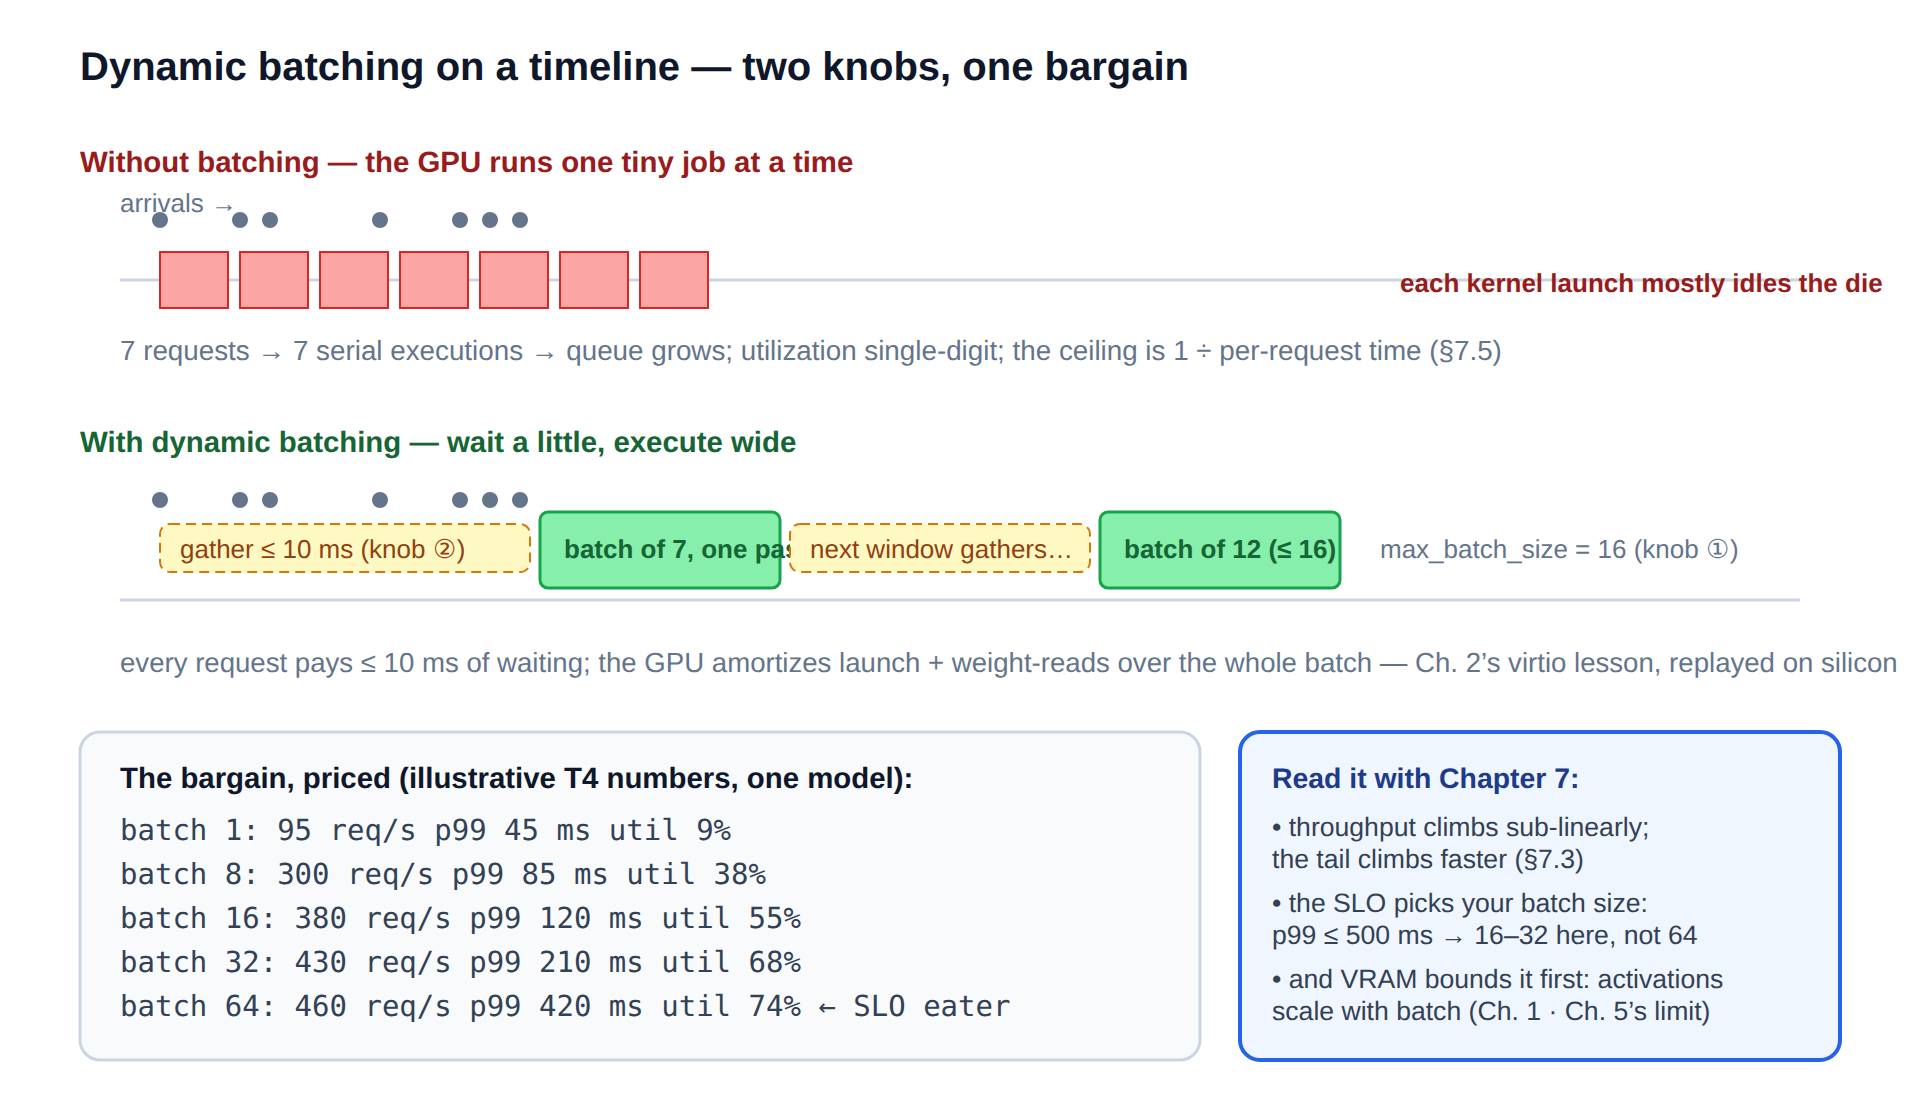
\includegraphics{figures/fig9-3_batching.png}}\\[3pt]
  \figcaption{그림 9-3  시간축으로 본 동적 배치 처리. 최대 배치 크기와 최대 대기열 지연이라는 두 설정값과 절충 관계의 가격을 보여 준다. 처리량은 선형보다 느리게 늘고 꼬리는 더 빠르게 늘며 SLO가 운영 지점을 고른다.}
\end{tbbfigure}

\subsection*{두 설정값과 결정 주체}

동적 배처는 정확히 두 가지 약속을 지키며 두 상한으로 표현한다. \textbf{max\_batch\_size}는 실행 \textit{너비}의 상한이다. 취향이 아니라 \textbf{VRAM}이 결정한다. 활성화 메모리는 배치와 함께 늘어나므로(제1장의 급증 교훈) 실제 상한은 "가중치 옆에 들어가는 가장 큰 배치 × 가장 긴 입력"이다. 제5장에서 \code{memory.max} 기반 상한을 설정하기 전에 측정하라고 한 최악의 경우와 정확히 같다. §9.5의 Locust 실행으로 의도적으로 생성한다. \textbf{max\_queue\_delay}는 첫 요청이 동료를 얼마나 \textit{오래} 기다릴지 제한한다. 이 설정값은 \textbf{SLO가 기계적으로} 정한다. p99 ≤ 500 ms이고 배치 계산 비용이 \textasciitilde{}35 ms라면 10 ms 수집 구간은 예산의 2\%를 써 \textasciitilde{}20× 처리량을 얻는다(그림 9-1의 계산). 100 ms 구간은 작업이 시작되기도 전에 예산의 5분의 1을 쓴다. 부하가 크면 배치가 즉시 차므로 지연 설정은 거의 영향을 주지 않는다. \textit{가벼운 부하}의 최악을 제한하기 위해 존재한다. 새벽 3시의 외로운 요청이 오지도 않을 동료를 구간 끝까지 기다려서는 안 된다.

실습에서 사용할 Triton의 설정 언어로 이 절 전체를 표현하면 여섯 줄이다. 바로 그것이 핵심이다.

\begin{terminalbox}
\begin{Verbatim}[breaklines=true,breakanywhere=true,fontsize=\small,formatcom=\color{tbbtermfg},codes=\tbbcodeactive]
$ cat model_repository/resnet50/config.pbtxt
platform: "onnxruntime_onnx"        # §7.6's format, meeting its runtime
max_batch_size: 32
dynamic_batching {
  preferred_batch_size: [ 8, 16 ]
  max_queue_delay_microseconds: 10000     # 10 ms: 2% of the SLO budget
}
instance_group [ { count: 2, kind: KIND_GPU } ]   # organ ③: pipelining
# eight months of Exhibit 9-B, expressed as configuration.
\end{Verbatim}
\end{terminalbox}
\figcaption{터미널 기록 9-2  설정으로 표현한 절충 관계. max\_batch\_size는 VRAM이 제한하므로 최악의 경우를 측정하고, max\_queue\_delay는 SLO가 정하므로 지연 시간 예산의 작고 알려진 몫을 쓰며, instance\_group은 파이프라이닝을 산다.}

\subsection*{엔지니어처럼 절충 관계 읽기}

그림 9-3의 가격표는 제7장의 관점으로 읽을 때 의미가 커진다. 배치 처리는 커널 실행과 가중치 읽기 비용을 분산하지만 계산 자체는 줄이지 못하므로 처리량은 1 → 64에서 95 → 460 req/s로 \textbf{선형보다 느리게} 늘어난다. 표 중간을 지나면 꼬리가 \textbf{처리량보다 빠르게} 늘어난다. 큰 배치에서는 함께 묶인 모든 요청이 가장 넓고 느린 실행을 기다리기 때문이다. 배치는 작은 팬아웃이고 §7.3에서 모두 기다릴 때 꼬리에 일어나는 일을 배웠다. 따라서 운영 지점은 "들어가는 가장 큰 배치"가 아니라 \textbf{"목표 부하에서 p99가 여전히 SLO를 지키는 가장 큰 배치"}다. 표에서는 500 ms 약속에 16–32가 해당하며, 꼬리를 두 배로 늘려 처리량 7\%를 더 얻는 64는 분명 아니다. 솔직한 사실을 하나 더 보자. 동적 배치 처리는 \textit{동시} 트래픽에 도움이 된다. 사용자 하나의 조금씩 들어오는 요청은 배치를 만들지 못하고 지연 구간 비용만 낸다. 그래서 배치 크기 히스토그램이 메트릭 엔드포인트에 있어야 한다(§9.2 생각해 볼 문제). 트래픽 구성이 바뀌면 배처 효과도 조용히 달라진다.

\subsection*{두 매개변수로 설명하는 전체 표 — 기억할 만한 모델}

그림 9-3의 다섯 행은 경험적 결과처럼 보이지만 기억할 만큼 단순한 법칙이 숨어 있다. 배치 실행 하나의 시간을 \textbf{t(B) = a + b·B}로 모델링하자. \textit{a}는 실행마다 한 번 내는 고정 비용(커널 실행, 스케줄링, 가중치 읽기)이고 \textit{b}는 배치 항목마다 내는 한계 비용(입력마다 실제로 해야 하는 계산)이다. 표에 맞추면 a ≈ 8.4 ms, b ≈ 2.05 ms가 나오고 모든 숫자가 재현된다. t(1) ≈ 10.5 ms → 95 req/s, t(16) ≈ 41 ms → 380 req/s, t(64) ≈ 140 ms → 460 req/s다. 대수에서 세 결과가 나온다. \textbf{상한은 1/b}로 여기서는 ≈ 488 req/s이며 어떤 배치 크기도 도달하지 못한다. 배치 처리는 \textit{a}를 분산하지만 \textit{b}는 건드리지 못해 곡선이 포화한다. \textbf{이익은 a/b}다. 고정 비용이 한계 비용보다 훨씬 크면(작은 모델, 큰 가중치, 빠른 GPU) 배치 처리가 놀라운 효과를 내고, \textit{b}가 지배하면(항목별 계산이 큼) 이익이 적어 다른 곳에 투자해야 한다. \textbf{10주 차에는 두 상수를 직접 공격한다.} 컴파일(TensorRT)은 커널을 융합해 \textit{a}를 줄이고, 양자화는 계산을 저렴하게 해 \textit{b}를 줄인다. 그래서 다음 주 벤치마크 실습에서 정확히 이 스윕을 다시 실행하고 두 숫자를 다시 적합한다. 실습에서 자기 모델의 a와 b를 측정하면(배치 1과 배치 32 두 번이면 충분) Locust가 확인하기 전에 전체 처리량 곡선을 예측할 수 있다.

\begin{calloutbox}{tbbteal}{tbbtealfill}
{\normalsize\bfseries\color{tbbx115E59}상자 9-1  배치 처리 이야기가 이어지는 곳}\par\vspace{3pt}
\textbf{이 장:} 이미지 분류기, 임베딩 모델, 랭커처럼 독립적이고 형태가 비슷한 요청의 동적 배치 처리를 다룬다. 요청 하나가 단위 하나이며 배치 처리는 투명하다.

\textbf{11주 차:} LLM 생성은 "형태가 비슷하다"는 가정을 치명적으로 깨뜨린다. 시퀀스마다 길이와 종료 시점이 다르므로 고전 동적 배치 처리는 가장 긴 시퀀스를 기다리며 GPU 절반을 비운다. 해결책인 토큰마다 배치에 들어오고 나가는 \textbf{연속 배치 처리}와 이를 가능하게 하는 KV 캐시가 vLLM의 존재 이유다. 그림 9-4에서 일반 프레임워크 지도 밖에 둔 이유이기도 하다.
\end{calloutbox}

\vspace{3.0pt}

\begin{calloutbox}{tbbpurple}{tbbpurplefill}
{\normalsize\bfseries\color{tbbpurple}생각해 보기}\par\vspace{3pt}
\begin{tbbitemize}
  \item 모델의 배치 계산은 배치 16에서 35 ms가 들고 SLO는 게이트웨이에서 측정한 p99 ≤ 200 ms로 진행 예보다 엄격하다. 네트워크 + 게이트웨이 + 전처리(\textasciitilde{}40 ms, 제6장)를 고려해 대기열 지연 설정 예산을 잡자. 방어할 수 있는 가장 큰 max\_queue\_delay는 얼마인가?
  \item 팀원이 배치 64를 "최고 처리량"으로 벤치마크하고 프로덕션에 max\_batch\_size = 64를 설정한다. 밤 트래픽의 40\%는 단일 사용자의 간헐적 요청이다. 이 설정이 실망을 주는 서로 다른 두 방식인 가격표의 꼬리 열과 간헐적 요청 문제를 설명하고 대신 설정할 값을 제안하자.
  \item 인스턴스 그룹(count: 2)은 배치 처리 \textit{없이도} 사례 9-A 형태 서버의 처리량을 거의 두 배로 늘렸다. §9.2의 기관 ③을 사용해 메커니즘을 한 문장으로 설명하고 count: 8이 8×를 주지 못하는 이유를 말하자. 복사본이 공유하는 리소스는 무엇인가?
\end{tbbitemize}
\end{calloutbox}

\section{대표 프레임워크 네 가지 — 같은 기관, 네 철학}

이제 제품을 보자. 강의계획서에는 \textbf{Triton Inference Server, TorchServe, BentoML, Ray Serve} 네 가지가 나온다. 혼동을 멈추는 가장 빠른 방법은 같은 여섯 기관을 바라보는 네 가지 \textit{견해}이며 두 축에서 다르다고 보는 것이다(그림 9-4). 무게 중심이 아티팩트 하나를 최대한 강하게 서빙하는 \textbf{모델 엔진}에 있는가, 모델과 로직을 조합하는 \textbf{애플리케이션 프레임워크}에 있는가가 첫 축이다. \textbf{설정}으로 구동하는 운영 우선 방식인가, \textbf{코드}로 구동하는 Python 우선 방식인가가 두 번째 축이다. 지도에 프레임워크를 놓으면 문서 대부분을 예측할 수 있다.

\begin{tbbfigure}
  \adjustbox{max width=0.94\linewidth,max totalheight=0.46\textheight}{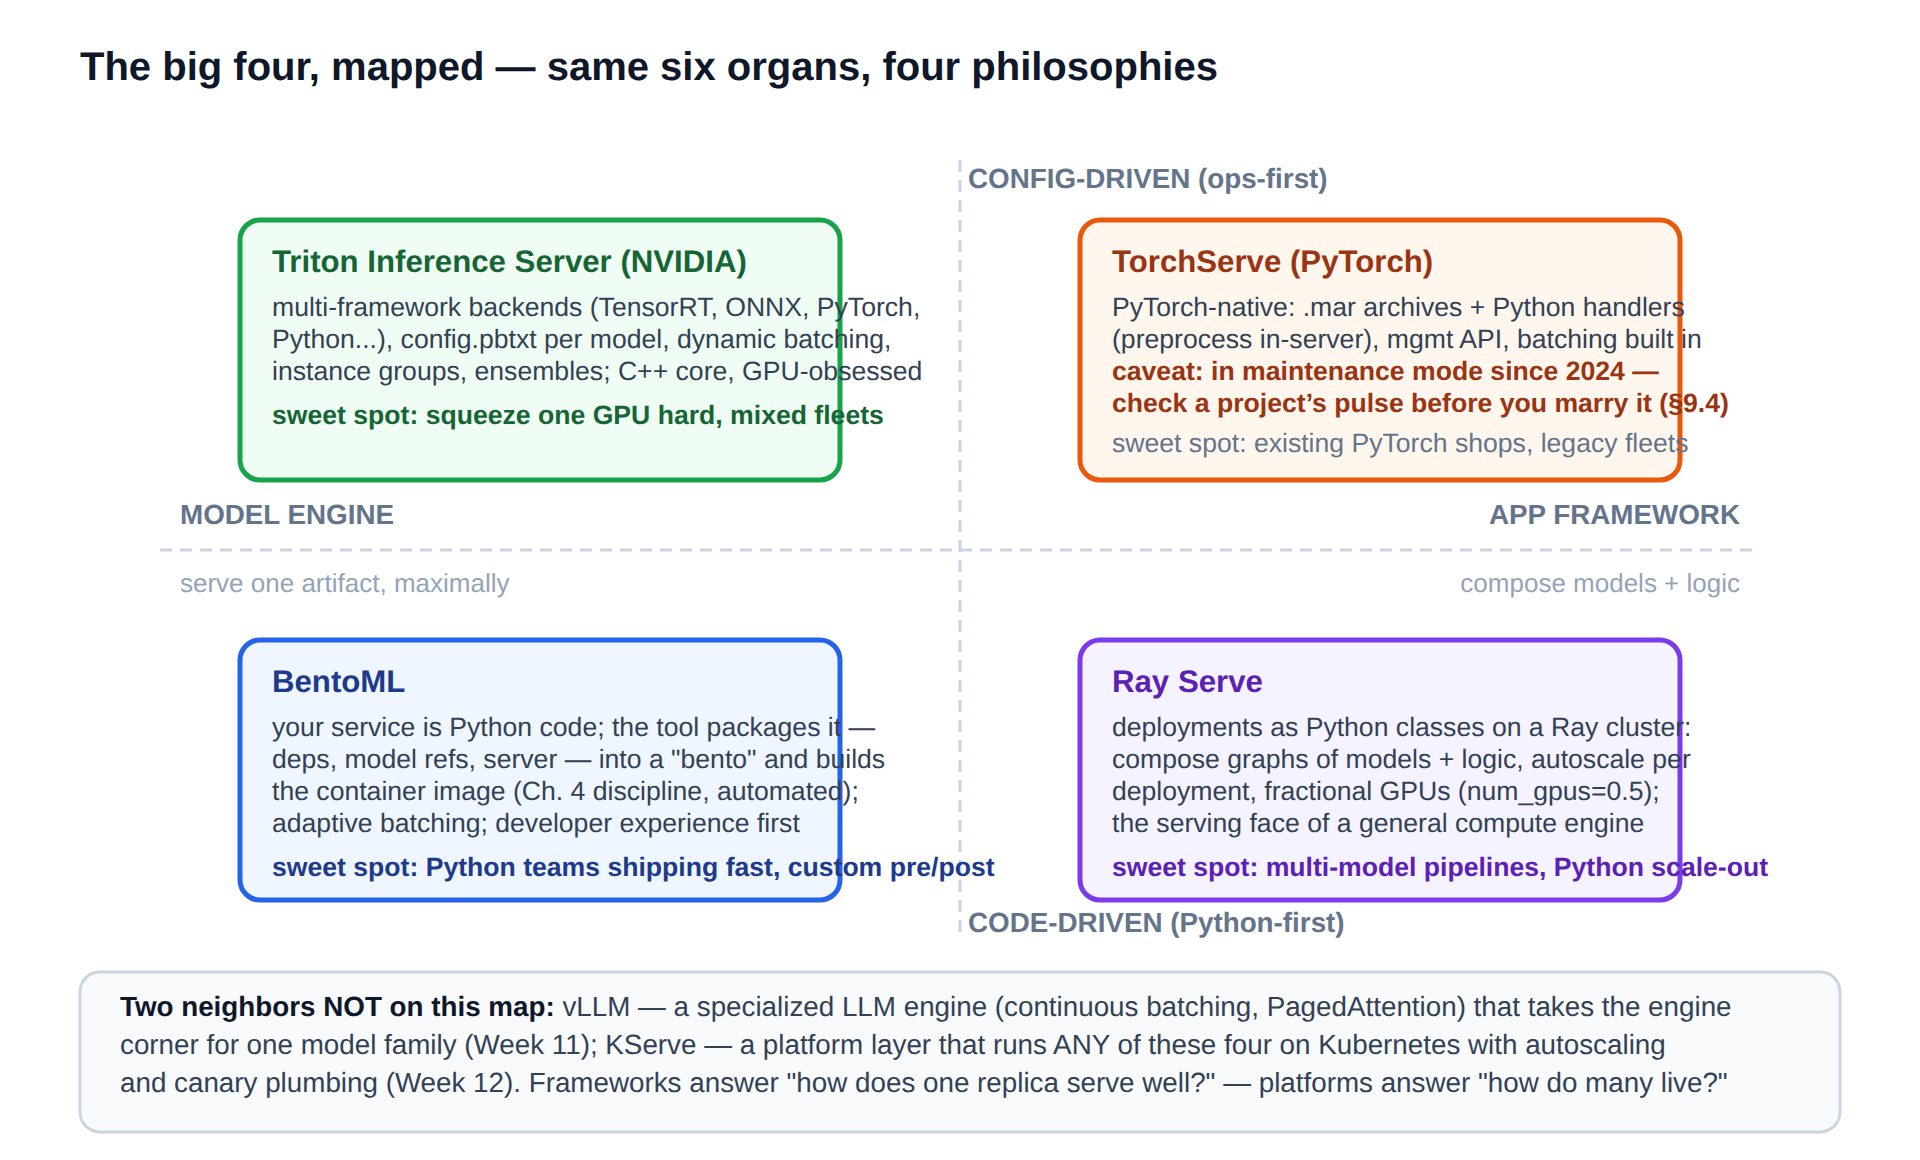
\includegraphics{figures/fig9-4_map.png}}\\[3pt]
  \figcaption{그림 9-4  두 축에 놓인 대표 프레임워크 네 가지. LLM 전문 엔진인 vLLM(11주 차)과 어느 프레임워크든 Kubernetes에서 실행하는 플랫폼인 KServe(12주 차)는 의도적으로 지도 밖에 두었다.}
\end{tbbfigure}

\subsection*{Triton: GPU를 끝까지 활용하는 설정 우선 엔진}

\textbf{Triton}(NVIDIA, 2018년 TensorRT Inference Server로 탄생해 2020년 이름 변경)은 엔진 영역을 진지하게 밀어붙인 모습이다. C++ 서버의 \textbf{백엔드}가 §7.6에서 만든 TensorRT 엔진, 실습에서 사용할 ONNX, TorchScript, 임의의 Python까지 통일된 API 뒤에서 모델 하나 또는 수백 개를 나란히 실행한다. 모든 것은 모델 저장소와 \code{config.pbtxt}(터미널 기록 9-2)로 표현한다. 동적 배치 처리, 인스턴스 그룹, 버전 정책을 코드가 아니라 선언으로 지정한다. 강력한 기능도 GPU에 집착하는 엔진다운 것들이다. 클라이언트 왕복 없이 전처리 → 모델 → 후처리를 실행하는 서버 측 DAG인 \textbf{앙상블}, 분리형/스트리밍 응답, 배치 크기와 동시성을 대신 스윕하는 내장 부하 생성기 \code{perf\_analyzer}를 제공한다. 명확한 철학을 지닌 Locust 형태 도구로 실습에서는 둘 다 쓴다. 이 모든 것의 비용은 철학에 있다. 전처리/후처리는 앙상블 안의 모델(Python 백엔드의 "모델")이 되거나 클라이언트에 있거나 존재하지 않아야 한다. Triton은 애플리케이션 코드를 서버 밖에 두기를 선호한다. 저장소 배치는 다음과 같다.

\begin{terminalbox}
\begin{Verbatim}[breaklines=true,breakanywhere=true,fontsize=\small,formatcom=\color{tbbtermfg},codes=\tbbcodeactive]
$ tree model_repository/          # local dir or s3://models/prod (Ch. 6)
model_repository/
└── resnet50/
    ├── config.pbtxt
    ├── 1/model.onnx              # version 1, kept for rollback
    └── 2/model.onnx              # version 2, live (policy: latest)
$ curl -s localhost:8000/v2/models/resnet50/versions/2/ready
{"ready": true}                    # organ ⑥, speaking K8s's language
# metrics on :8002/metrics, gRPC on :8001 - organs ⑤ and ①, batteries included.
\end{Verbatim}
\end{terminalbox}
\figcaption{터미널 기록 9-3  Triton의 모델 저장소. 하나의 접두사 아래 버전을 나란히 두어 제6장의 선반을 그대로 사용하고 제13장의 롤백 이야기를 미리 연결해 놓았다.}

\subsection*{TorchServe: PyTorch 네이티브 베테랑과 생명력에 관한 교훈}

\textbf{TorchServe}(AWS + Meta, 2020)는 PyTorch 색채가 있는 엔진 영역이다. \code{torch-model-archiver}로 가중치와 서버 안에서 실행할 전처리/후처리 Python \textbf{핸들러}를 \code{.mar} 아카이브로 패키징하면 서버가 배치 처리, 버전이 있는 관리 API, 메트릭 같은 기관을 제공한다. 오랫동안 "PyTorch 모델이 있다"에 대한 기본 답이었고 바로 그 이유로 현장에서 만날 것이다. 이 절의 경고 사례도 담고 있다. 2024년 프로젝트가 \textbf{유지 관리 모드}에 들어가 기능은 유지하지만 적극적으로 개발하지 않게 되었다. 교훈은 "TorchServe가 나쁘다"가 아니다. \textbf{프레임워크에는 맥박이 있으므로 결혼하기 전에 확인해야 한다.} 릴리스 주기, 이슈 분류, 유지 관리자의 고용 주체를 살펴본다. 탈출 비용도 낮게 유지해야 한다. §7.6은 \textit{아티팩트}를 개방형 형식으로 보관하라고 했고 §9.2는 기관이 보편적이라고 했다. 따라서 TorchServe 플릿을 Triton 또는 후속 제품으로 옮기는 일은 작업이지만 재앙은 아니다. 비즈니스 로직을 프레임워크 내부와 결합한 팀은 그 차이를 비싸게 배웠다.

\subsection*{BentoML: 코드 우선 패키징 도구}

\textbf{BentoML}은 다른 개발자에게 답한다. \textit{"서비스가 Python이고 모델, 약간의 전처리/후처리, 어쩌면 모델 두 개와 규칙 하나가 있다. 이를 배포하고 싶다."} 형식이 지정된 엔드포인트가 있는 일반 Python 클래스를 작성하면 BentoML이 주위에 서버, 적응형 배치 처리, 메트릭 같은 기관을 제공한다. 대표 동작은 \textbf{전체를 패키징하는 것}이다. \code{bentoml build}가 코드, 의존성, 모델 참조를 버전이 있는 "bento"로 만들고 \code{bentoml containerize}가 Docker 이미지를 내보낸다. 마지막 단계는 익숙할 것이다. 사례 4-A에서 극적으로 보여 준 제4장의 규율인 의존성 고정, 계층형 이미지, "내 컴퓨터에서는 됨" 제거를 자동화한다. 도구로 만든 안전장치다. 절충 관계는 Triton의 거울상이다. Triton이 최대한 선언적인 곳에서 BentoML은 최대한 표현력이 높지만 GPU를 끝까지 활용하는 상한과 운영팀의 가독성에서 비용을 낸다. 철학을 여덟 줄로 보면 다음과 같다.

\begin{terminalbox}
\begin{Verbatim}[breaklines=true,breakanywhere=true,fontsize=\small,formatcom=\color{tbbtermfg},codes=\tbbcodeactive]
# service.py - the service IS this class; the organs wrap it
import bentoml

@bentoml.service(resources={"gpu": 1})
class Classifier:
    def __init__(self):                    # organ ⑥: load = ready
        self.model = load_onnx("clf:v7")   # from the bento's models

    @bentoml.api(batchable=True, max_batch_size=16,
                 max_latency_ms=10)         # §9.3's two knobs, as kwargs
    def classify(self, images: list) -> list:
        return self.model.run(preprocess(images))   # YOUR code, in-server
$ bentoml build && bentoml containerize clf:latest   # Ch. 4, automated
\end{Verbatim}
\end{terminalbox}
\figcaption{터미널 기록 9-4a  BentoML의 철학. 서비스는 일반 Python이고 배치 처리 설정값은 데코레이터 인수이며 고정된 컨테이너 이미지로 패키징하는 일은 하위 명령이다.}

\subsection*{Ray Serve: 분산 프로그램으로서의 서빙}

\textbf{Ray Serve}는 코드 우선 철학을 바깥으로 확장한다. \textbf{배포 단위}는 Ray 클러스터 전체에 배치하는 Python 클래스이며 각각 자체 레플리카 수, 리소스 요청, 오토스케일링 정책이 있다. \textbf{분할 GPU}도 지원해 \code{num\_gpus=0.25}로 작은 모델 네 개가 카드 하나를 공유할 수 있다. 제2장의 공유 이야기를 프레임워크 계층에서 구현했으며 이웃을 하드웨어로 격리하지 못한다는 같은 주의사항이 따른다. 일반 메서드 호출로 배포 단위를 그래프로 조합한다. 서빙 \textit{자체가} 검색 → 순위화 → 필터링 → 생성처럼 각 단계가 독립적으로 확장하는 애플리케이션이거나 팀이 이미 데이터와 학습에 Ray를 쓸 때 자연스러운 답이다. 비용은 이제 Ray 클러스터를 운영한다는 것이다. Kubernetes 위에 사는 두 번째 스케줄러로 제5장의 "두 두뇌" 패턴이다. 강력하지만 호출기를 울릴 대상이 하나 더 생긴다.

\begin{terminalbox}
\begin{Verbatim}[breaklines=true,breakanywhere=true,fontsize=\small,formatcom=\color{tbbtermfg},codes=\tbbcodeactive]
# app.py - an application of models, composed and scaled per stage
from ray import serve

@serve.deployment(num_replicas=2, ray_actor_options={"num_gpus": 0.25})
class Reranker: ...                        # a quarter of a GPU each

@serve.deployment(autoscaling_config={"min_replicas": 1,
                                      "max_replicas": 8})
class Retriever: ...                       # scales on ITS own load

@serve.deployment
class QueryPath:                           # the graph: plain method calls
    def __init__(self, retriever, reranker):
        self.r, self.rr = retriever, reranker
    async def __call__(self, q):
        return await self.rr.rank.remote(await self.r.fetch.remote(q))
\end{Verbatim}
\end{terminalbox}
\figcaption{터미널 기록 9-4b  Ray Serve의 철학. 각 단계는 자체 레플리카, GPU 할당 비율, 오토스케일링을 가진 배포 단위다. 설정한 서버가 아니라 분산 Python 프로그램으로 서빙한다.}

\begin{tbbtablewrap}
  \begin{tabular}{@{}>{\raggedright\arraybackslash}m{\dimexpr 0.1915\tbltextwidth-2\tabcolsep\relax} >{\raggedright\arraybackslash}m{\dimexpr 0.2074\tbltextwidth-2\tabcolsep\relax} >{\raggedright\arraybackslash}m{\dimexpr 0.1968\tbltextwidth-2\tabcolsep\relax} >{\raggedright\arraybackslash}m{\dimexpr 0.1968\tbltextwidth-2\tabcolsep\relax} >{\raggedright\arraybackslash}m{\dimexpr 0.2074\tbltextwidth-2\tabcolsep\relax}@{}}
  \arrayrulecolor{tbbnavy}\specialrule{1pt}{0pt}{0pt}
  \rowcolor{tbbtablehead}{\centering \bfseries\color{tbbnavy} } & {\centering \bfseries\color{tbbnavy}Triton} & {\centering \bfseries\color{tbbnavy}TorchServe} & {\centering \bfseries\color{tbbnavy}BentoML} & {\centering \bfseries\color{tbbnavy}Ray Serve} \\
  \arrayrulecolor{tbbnavy}\specialrule{0.7pt}{0pt}{2pt}
  {\textbf{배포 대상}} & {모델 저장소(설정 기반)} & {.mar 아카이브 + 핸들러} & {"bento"(코드 + 의존성 + 모델)} & {Ray 클러스터의 Python 배포 단위} \\
  \arrayrulecolor{tbbtableborder}\hline
  {\textbf{전처리/후처리 위치}} & {클라이언트 또는 앙상블/Python 백엔드} & {서버 내부 핸들러} & {서비스 코드} & {배포 단위 코드} \\
  \arrayrulecolor{tbbtableborder}\hline
  {\textbf{배치 처리}} & {동적, 선언형, 모델별} & {내장형, 모델별} & {적응형, 엔드포인트별} & {배포 단위별(@serve.batch)} \\
  \arrayrulecolor{tbbtableborder}\hline
  {\textbf{형식}} & {TensorRT · ONNX · TorchScript · Python… (§7.6 선택지)} & {PyTorch 계열} & {Python이 로딩할 수 있는 모든 것} & {Python이 로딩할 수 있는 모든 것} \\
  \arrayrulecolor{tbbtableborder}\hline
  {\textbf{여러 모델}} & {서버마다 수백 개, 앙상블} & {여러 개, 관리 API} & {서비스별 조합} & {배포 단위 그래프} \\
  \arrayrulecolor{tbbtableborder}\hline
  {\textbf{주의점}} & {애플리케이션 로직을 서버 밖에 두기} & {유지 관리 모드의 맥박(2024)} & {GPU 활용 상한} & {Ray 자체 운영} \\
  \arrayrulecolor{tbbtableborder}\hline
  {\textbf{적합한 곳}} & {GPU 극대화, 혼합 형식 플릿, 운영팀이 관리하는 플랫폼} & {기존 PyTorch 조직, 레거시 플릿} & {빠르게 배포하는 Python 팀} & {다중 모델 파이프라인, Ray 조직} \\
  \arrayrulecolor{tbbnavy}\specialrule{1pt}{2pt}{0pt}
  \end{tabular}\par
  \figcaption{표 9-2  대표 프레임워크 네 가지 한눈에 보기}
\end{tbbtablewrap}

\subsection*{정직하게 선택하기}

그림 9-7은 결정을 네 질문으로 압축한다. 워크로드 형태가 인기 모델 하나인지 애플리케이션인지, 전처리/후처리가 어디에 살아야 하는지, 누가 운영하는지, 프로젝트가 살아 있고 탈출 비용이 낮은지를 묻는다. 이어 중요한 벤치마크 규칙은 하나뿐이다. \textbf{자기 모델, 자기 SLO, 자기 하드웨어에서 후보를 벤치마크한다.} 공개 막대 차트는 다른 사람의 모델, 배치 크기, "지연 시간" 정의로 만들었다. 배치 처리가 도움을 주고 엔진이 원시 처리량에서 프레임워크를 이긴다는 \textit{형태}는 옮겨 오지만 \textit{숫자}는 절대 그렇지 않다. §9.5 덕분에 자기 벤치마크를 오후 하나에 저렴하게 실행할 수 있다. 이 강의는 9주 차 실습에 \textbf{Triton}을 고른다. 동적 배치 처리를 눈에 보이게 하고 §7.6의 ONNX를 바로 넣을 수 있다. 코드 우선 팀을 위한 BentoML 경로도 있다. 11주 차에 연속 배치 처리가 양보할 수 없는 조건이 되면 \textbf{vLLM}이 이어받는다. 12주 차에는 \textbf{KServe}가 등장해 선택한 프레임워크를 클러스터에서 실행한다. 프레임워크는 \textit{레플리카 하나가 잘 서빙하는 방법}에, 플랫폼은 \textit{몇 개 레플리카가 살아야 하는지}에 답한다.

\begin{tbbfigure}
  \adjustbox{max width=0.94\linewidth,max totalheight=0.46\textheight}{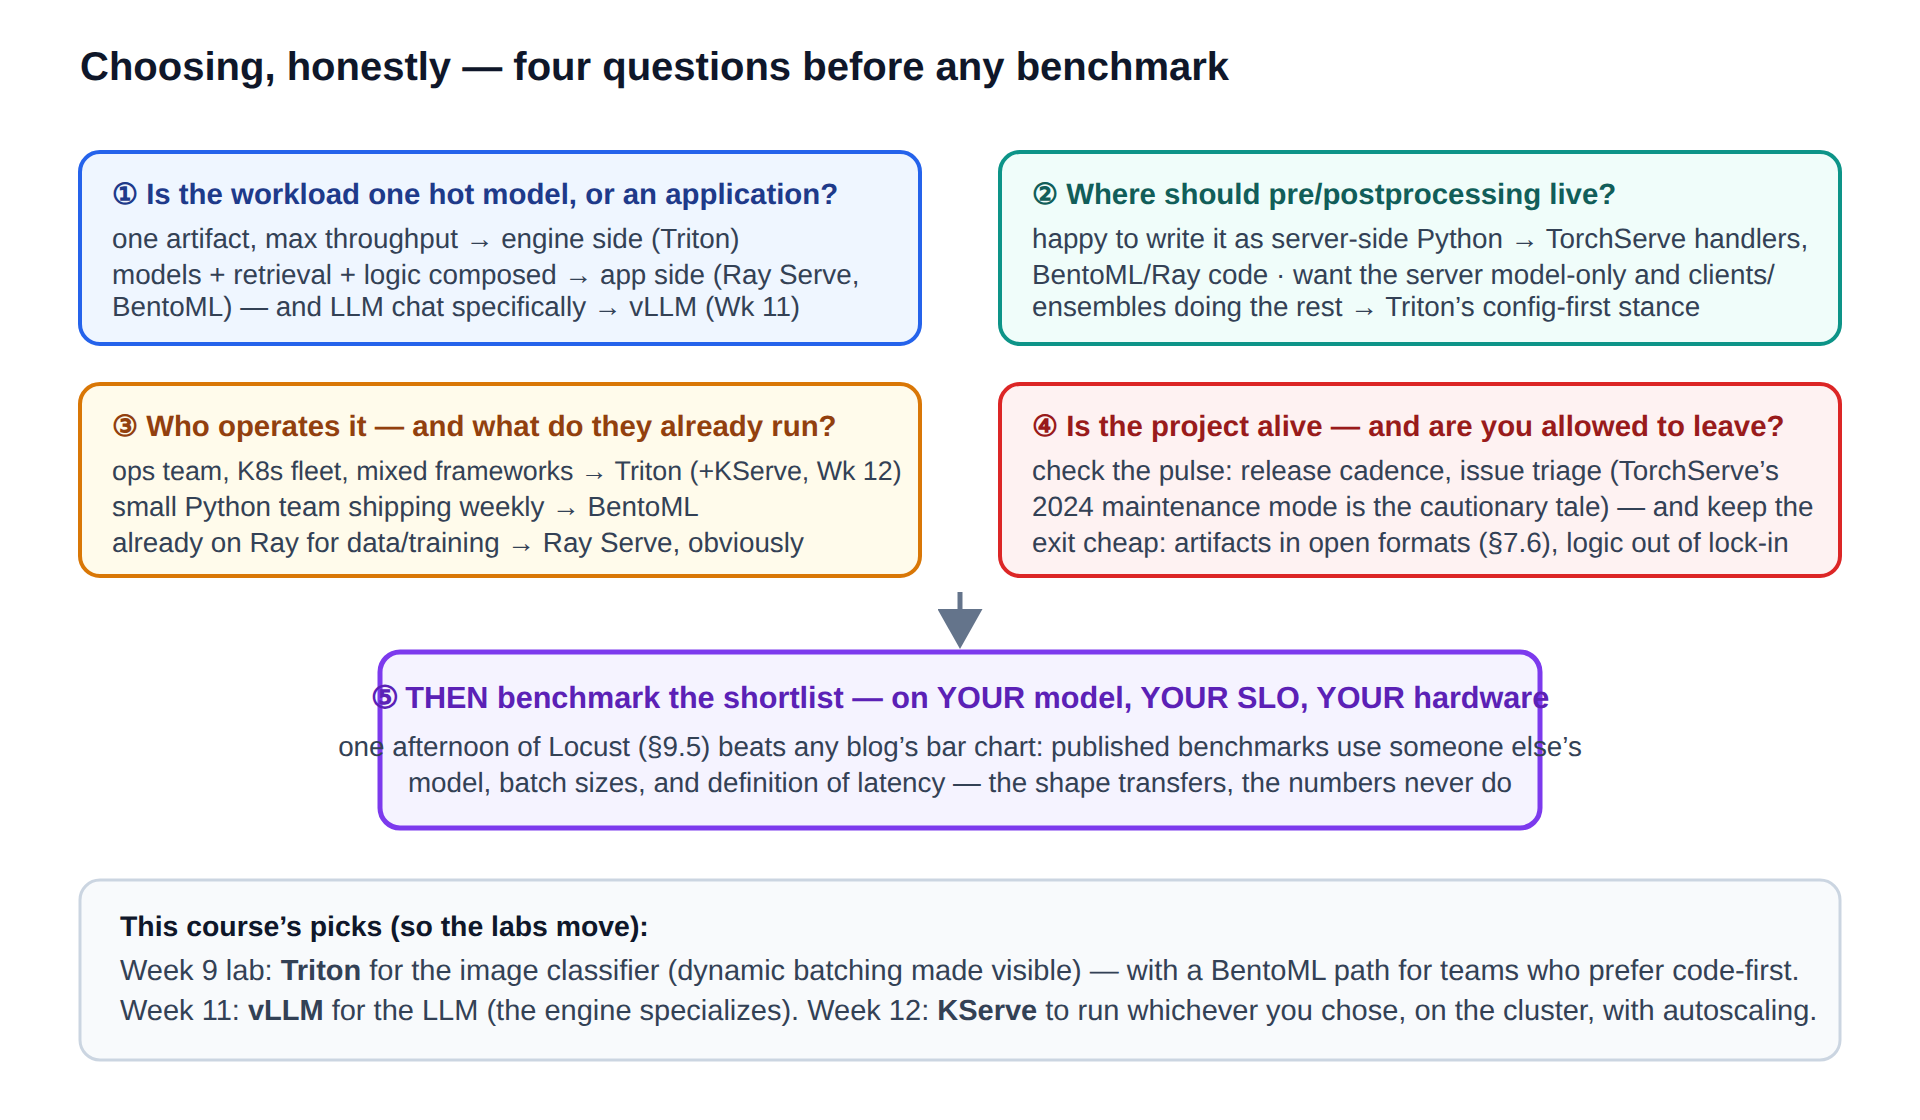
\includegraphics{figures/fig9-7_choose.png}}\\[3pt]
  \figcaption{그림 9-7  선택 체크리스트. 네 질문 뒤에 자기 워크로드에서 후보를 벤치마크한다. 아래에는 실습을 진행하기 위한 이 강의의 선택을 표시했다.}
\end{tbbfigure}

\begin{calloutbox}{tbbpurple}{tbbpurplefill}
{\normalsize\bfseries\color{tbbpurple}생각해 보기}\par\vspace{3pt}
\begin{tbbitemize}
  \item 세 팀을 그림 9-4에 놓고 각각의 선택을 옹호하자. (a) ML 엔지니어 두 명, 미세 조정한 비전 모델 하나, 월 30\% 성장하는 트래픽, (b) 공유 GPU 풀에서 여섯 팀의 모델 40개를 실행하는 플랫폼 팀, (c) 쿼리 경로가 검색 → 재순위화 → 필터링이고 색인에 이미 Ray를 쓰는 검색 팀이다.
  \item 회사가 2022년에 TorchServe를 표준화했고 지금은 2026년이다. 무엇이 바뀌었는지(§9.4의 맥박 교훈), 무엇이 보호하는지(§7.6 + §9.2), 처음 벤치마크할 대상을 포함해 어떤 마이그레이션을 제안할지 세 줄 메모로 작성하자.
  \item Triton은 전처리를 서버 밖으로 밀고 TorchServe와 BentoML은 안으로 끌어들인다. 실습의 이미지 분류기에서 (a) GPU 사용률, (b) 클라이언트 단순성, (c) 꼬리 지연 시간 측면에서 어느 배치가 이기는가? 사례 9-A의 60 ms가 실제로 어디에 쓰였는지 떠올리자.
\end{tbbitemize}
\end{calloutbox}

\section{Locust: 중요한 숫자를 제대로 측정하기}

제7장은 정직한 측정을 법으로 정했다(상자 7-1). 이 절에서는 실습 부하 도구인 \textbf{Locust}로 구현한다. Python 네이티브이고 스크립트로 제어할 수 있으며 순진하게 사용하기 전까지는 쾌적하다. 함정은 §7.3에서 이름 붙인 것이다. Locust 사용자는 기본적으로 \textbf{폐쇄 루프}라 각각 응답을 기다린 뒤 다시 보낸다. 별도로 설정하지 않은 부하 집단은 서버가 힘들어하는 바로 그때 정중하게 느려지고 조정 누락이 조용히 백분위수를 편집한다. 해결책은 한 줄이며 파일에서 가장 중요한 줄이다.

\begin{terminalbox}
\begin{Verbatim}[breaklines=true,breakanywhere=true,fontsize=\small,formatcom=\color{tbbtermfg},codes=\tbbcodeactive]
$ cat locustfile.py
from locust import HttpUser, task, constant_throughput

class Client(HttpUser):
    # THE line: each user fires 2 req/s on a fixed clock,
    # whether or not replies come back -> arrivals never pause.
    wait_time = constant_throughput(2)

    @task
    def classify(self):
        with self.client.post("/v2/models/resnet50/infer",
                data=PAYLOAD, catch_response=True, timeout=2.0) as r:
            if r.elapsed.total_seconds() > 0.5:   # the SLO, enforced
                r.failure("over SLO")             # -> goodput, not throughput

# offered load = users x 2 req/s: sweep by stepping -u 60,90,120,135...
$ locust -f locustfile.py --headless -u 120 -r 20 --run-time 4m ...
\end{Verbatim}
\end{terminalbox}
\figcaption{터미널 기록 9-5  상자 7-1을 따르는 locustfile. constant\_throughput 페이싱(개방 루프 도착), 코드 안에서 강제하는 SLO(SLO 초과 응답을 실패로 세어 구조적으로 유효 처리량 계산), 사용자 수의 단계별 조정으로 부하 스윕을 구현한다.}

세 가지 습관이 방법을 완성한다. \textbf{사용자를 충분히 프로비저닝한다.} 제공 부하는 사용자 수 × 사용자당 요청률이며 각 사용자는 평균적으로 rate × timeout ≤ 1 request outstanding이어야 한다. 사용자가 너무 적으면 변장한 폐쇄 루프가 된다. 경험 법칙은 users ≥ 2 × target λ × worst-case latency다. \textbf{한 지점만 확인하지 말고 스윕한다.} 요청률 하나로는 변곡점을 알 수 없다. 의심하는 용량의 50/75/90/105/115\%를 단계별로 3분 이상 실행하고 첫 1분은 버린다(그림 9-5). \textbf{유효 처리량을 읽는다.} locustfile이 SLO 초과 응답을 실패 처리하므로 Locust 자체 실패 열이 \textit{곧} SLO 준수율이다. 사후 필터링도 없고 별도 표에 숨은 시간 초과도 없다.

\begin{tbbfigure}
  \adjustbox{max width=0.94\linewidth,max totalheight=0.46\textheight}{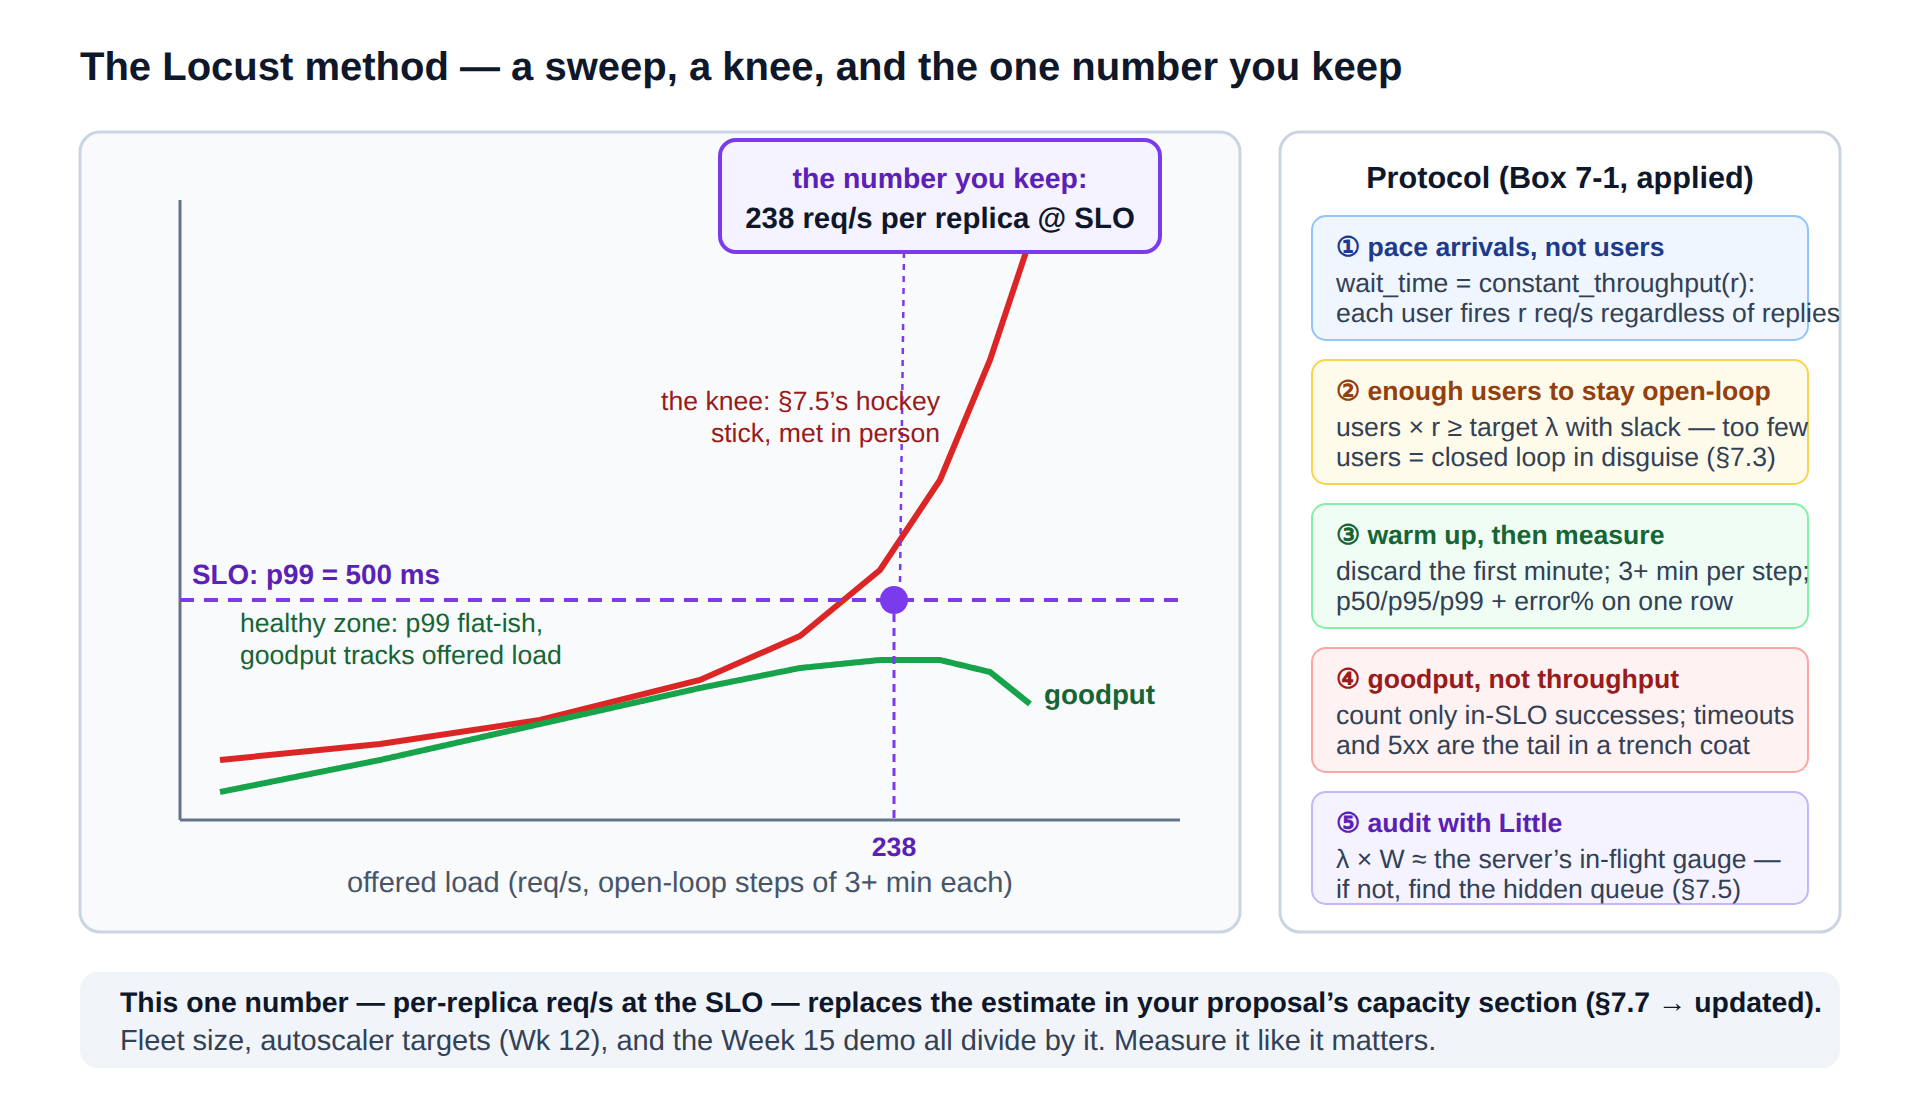
\includegraphics{figures/fig9-5_locust.png}}\\[3pt]
  \figcaption{그림 9-5  스윕, 변곡점, 그리고 유지할 숫자인 SLO에서 레플리카당 req/s. 프로토콜 패널은 상자 7-1을 적용한 것이며 숫자는 제안서 추정치를 대체한다.}
\end{tbbfigure}

\begin{terminalbox}
\begin{Verbatim}[breaklines=true,breakanywhere=true,fontsize=\small,formatcom=\color{tbbtermfg},codes=\tbbcodeactive]
# the sweep, tabulated (Triton, batching on, 1 replica, T4):
  offered   p50    p95    p99    err%   goodput   verdict
  120/s     58ms   96ms  145ms   0.0%   120/s     cruising
  180/s     66ms  118ms  190ms   0.0%   180/s     healthy
  240/s     84ms  168ms  310ms   0.2%   239/s     approaching knee
  260/s    118ms  290ms  520ms   1.9%   249/s     p99 breaches SLO
  290/s    460ms  1.9s   4.1s   11.4%   182/s     past the cliff:
                                                   goodput FALLING
# the number you keep: ~238 req/s at p99<=500ms. write it down.
# Little audit: 240/s x 0.084s = ~20 in flight; Triton's queue+exec
# gauges sum to 19-22 across the run. no hidden queue. (§7.5 ✓)
\end{Verbatim}
\end{terminalbox}
\figcaption{터미널 기록 9-6  스윕. 유효 처리량은 변곡점까지 제공 부하를 따라가다가 원시 처리량이 여전히 좋아 보이는 동안 감소한다. 리틀의 법칙 감사로 대시보드가 거짓말하지 않음을 확인한다. 238 req/s @ SLO를 제안서에 넣는다.}

\subsection*{의도적으로 만드는 재시도 폭풍 하나}

제6장은 재시도 논의를 약속으로 끝냈다. \textit{"9주 차 부하 테스트에서 재시도 폭풍을 의도적으로 보여 주어 파형을 알아보게 한다."} 이제 약속을 지킬 때다. 설정은 무해해 보인다. 수많은 HTTP 라이브러리의 기본값처럼 세 번 시도하고 백오프하지 않는 클라이언트 측 재시도를 locustfile에 추가하고 제공 부하를 변곡점보다 5\% 높여 2분 동안 밀어 넣는다. 결과인 그림 9-6은 오래 바라볼 가치가 있다. \textbf{3분째 사용자 수요는 정상으로 돌아오지만 시스템은 복구되지 않는다.} 시간 초과마다 재시도가 생기고 이미 용량을 넘은 서버의 도착 요청이 세 배가 된다. 추가 도착 요청이 더 많은 시간 초과를 만들며 루프가 닫힌다. 더 나쁘게도 서버의 처리 자리는 원래 클라이언트가 오래전에 연결을 끊은 작업으로 가득하다. 처리량은 \textit{바빠} 보이지만 유효 처리량은 0에 가깝다. 수요가 정상화된 뒤에도 도착 요청이 높게 고정되고 유효 처리량은 바닥에 붙는 징후가 재시도 폭풍이다. 이를 알아보지 못한 팀은 레플리카를 더해 "고친다." 쓰레기를 더 빨리 서빙하기 위해 3× 비용을 낸다.

\begin{tbbfigure}
  \adjustbox{max width=0.94\linewidth,max totalheight=0.46\textheight}{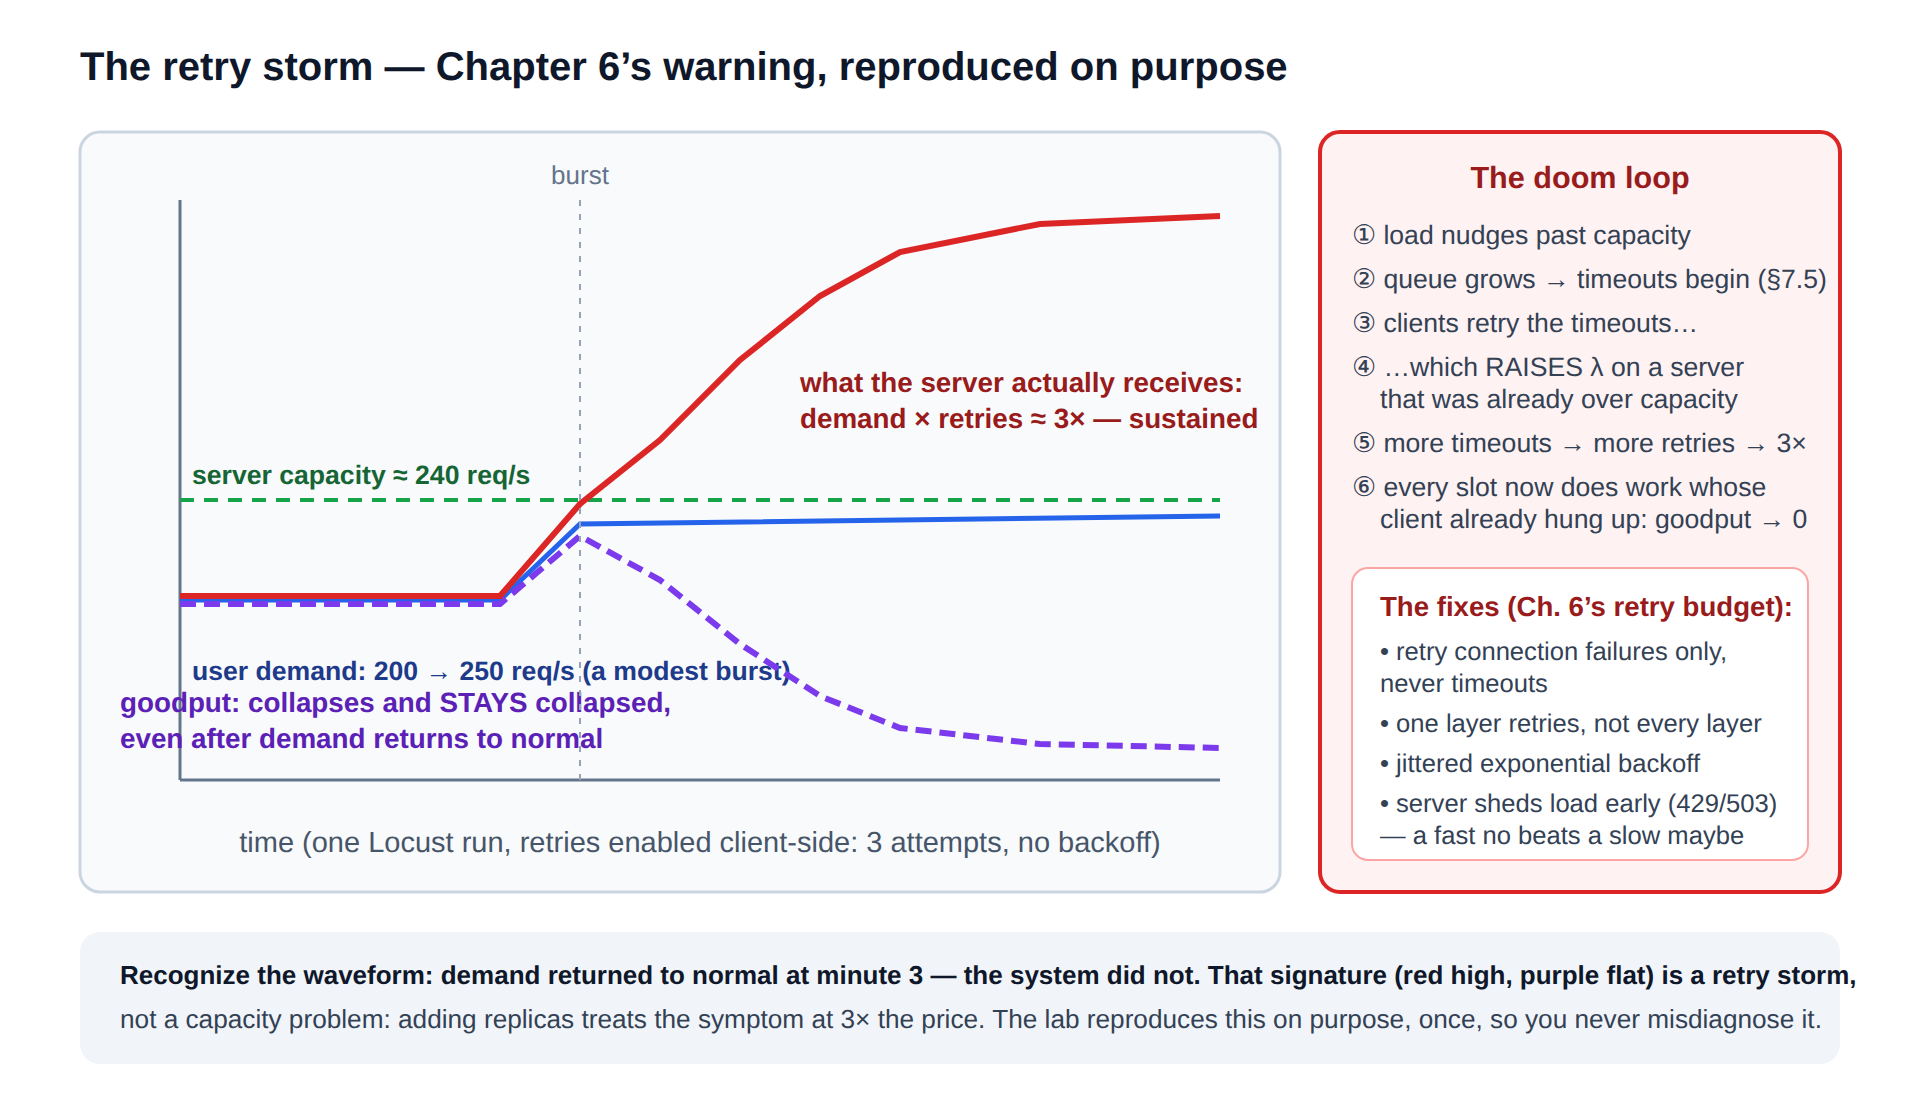
\includegraphics{figures/fig9-6_retrystorm.png}}\\[3pt]
  \figcaption{그림 9-6  재현한 재시도 폭풍. 변곡점 너머로 2분 밀어 넣기 + 순진한 클라이언트 재시도 = 지속되는 3× 도착 요청과 버스트보다 오래가는 유효 처리량 붕괴다. 해결책은 제6장의 재시도 예산 그대로다.}
\end{tbbfigure}

해결책은 이제 파형이 붙은 제6장의 재시도 예산이다. \textbf{연결 실패만 재시도하고 시간 초과는 절대 재시도하지 않는다.} 시간 초과는 서버가 요청을 가지고 있다는 뜻이므로 다시 보내면 순수한 증폭이다. \textbf{단일 계층만 재시도}한다. 클라이언트 \textit{또는} 게이트웨이 중 하나이며 둘이 곱하지 않는다. \textbf{지터를 적용한 지수 백오프}로 재시도가 동기화되지 않고 퍼지게 한다. 서버 자체의 방어는 \textbf{일찍 부하를 버리는 것}이다. 깊이 임계값을 넘으면 헛되이 대기열에 넣지 말고 즉시 429/503으로 거부한다. 빠른 \textit{거절}은 클라이언트가 백오프하게 하지만 느린 \textit{어쩌면}은 루프를 키운다. 429가 익숙해야 한다. 제1장의 울타리를 카운터 뒤에서 본 것이며 이제 양쪽에 서 보았다. 실습에서 폭풍을 한 번 실행하고 해결책을 적용해 다시 실행하면 같은 버스트를 가볍게 떨쳐 내는 모습을 볼 수 있다. Grafana 화면 캡처 두 장은 14주 차 새벽 2시에 파형을 다시 볼 때 산문 한 장보다 가치 있을 것이다.

\begin{calloutbox}{tbbpurple}{tbbpurplefill}
{\normalsize\bfseries\color{tbbpurple}생각해 보기}\par\vspace{3pt}
\begin{tbbitemize}
  \item 스윕의 최고 단계인 목표 290 req/s, 시간 초과 2.0 s에 사용자 프로비저닝 규칙을 적용하자. constant\_throughput(2)에 사용자가 몇 명 필요하며 사용자 150명만으로 실행하면 도착 과정에 어떤 일이 조용히 생기는가?
  \item 터미널 기록 9-6에서 290/s의 제공 부하에 대한 원시 처리량은 \textasciitilde{}205/s였다. 순진한 보고서는 자랑스럽게 인쇄할 숫자다. 유효 처리량이 182/s인 이유를 재구성하고 각 숫자가 §7.4의 어느 SLI에 해당하는지 말하자.
  \item 게이트웨이(제6장)는 5xx를 두 번 재시도하고 클라이언트 라이브러리는 시간 초과를 3번 재시도한다. 60초 성능 저하 동안 사용자 요청 하나가 서버 측 실행 몇 개가 될 수 있는가? 곱셈을 그린 뒤 "한 계층만 재시도" 규칙을 적용해 다시 계산하자.
\end{tbbitemize}
\end{calloutbox}

\section{실습: 서빙하고, 스윕하고, 의도적으로 폭풍 만들기}

실습에서는 강의 T4에서 이 장 전체를 조립한다. 또는 SLO를 낮춘 minikube + CPU를 사용해도 그림 9-1 각주처럼 형태는 유지된다. Triton으로 이미지 분류기를 서빙하고, 제7장의 방식으로 측정하며, 배치 처리 스위치를 켜 절충 거래가 일어나는 모습을 본 뒤, 통제된 재난 하나를 재현한다. 제출물은 스윕 표, GPU 사용률 화면 캡처 두 장, 폭풍과 수정의 전후 쌍, \textit{측정한} 숫자로 갱신한 제안서 용량 절이다.

\subsection*{여덟 단계}

\begin{tbbitemize}
  \item \textbf{① 패키징(§7.6 적용).} 스크립트에서 분류기를 ONNX로 내보내고 동등성 검사 묶음(eager와 허용 오차 + top-1 일치)을 실행한 뒤 모델 저장소를 구성한다. 자동화할 대상을 이해하도록 CI 변환 단계를 한 번 직접 수행한다.
  \item \textbf{② 선반에 올리기(제6장).} 저장소를 \code{s3:/\allowbreak /\allowbreak <team>/\allowbreak models/\allowbreak } 또는 로컬 MinIO에 푸시한다. Triton이 직접 읽는다. 자격 증명은 클러스터 내부 IRSA로 제공하고 이미지에 키를 넣지 않는다.
  \item \textbf{③ 배포(제5장).} 강의 Triton 매니페스트에서 \code{/\allowbreak v2/\allowbreak health/\allowbreak ready}에 준비 상태 프로브를 둔다. 모델이 예열될 때까지 트래픽을 막는 기관 ⑥이다. 제5장 방법에 따라 요청량/상한을 정한다. 먼저 최악의 경우(최대 배치 × 가장 큰 이미지)를 실행하고 \code{memory.max}를 설정하기 전에 \code{memory.current}를 읽는다. 종료 코드 137은 여전히 존재한다.
  \item \textbf{④ 기준선 스윕, 배치 처리 끄기.} \code{dynamic\_batching}이 없는 \code{config.pbtxt}, 터미널 기록 9-5의 locustfile로 다섯 단계를 실행해 표로 만든다. 변곡점에서 GPU 사용률을 기록한다. 사례 9-A 근처를 예상한다.
  \item \textbf{⑤ 배치 처리 켜기.} 터미널 기록 9-2의 여섯 줄을 추가하고 다시 스윕한다. 같은 실리콘과 새 표로 자기만의 그림 9-1을 만든다. 두 실행 모두 \code{nvidia-smi dmon}을 화면 캡처한다.
  \item \textbf{⑥ 설정값 하나 실험.} \code{instance\_group count: 1 → 2}로 바꾸고 한 번 다시 스윕한다. 배치 처리는 GPU 비용을 분산하고 인스턴스는 전처리/후처리를 계산과 겹친다(§9.2 기관 ③). \textit{이} 모델에서는 무엇이 더 중요했는지 설명한다.
  \item \textbf{⑦ 재시도 폭풍(§9.5).} 세 번 재시도/백오프 없음으로 변곡점의 1.1×에서 120초 실행하고 도착 요청 대 유효 처리량을 화면 캡처한다. 이어 재시도 예산을 적용한다. 시간 초과 재시도 제거, 지터를 적용한 백오프, Triton의 \code{max\_queue\_size} + \code{default\_timeout}을 통한 대기열 깊이 기반 부하 차단을 적용해 버스트를 반복하고 복구를 화면 캡처한다.
  \item \textbf{⑧ 제안서 갱신.} §7.7에서 추정한 레플리카별 요청률을 ⑤에서 측정한 숫자로 바꾼다. 플릿 규모와 월 청구서를 다시 계산한다(제2장 표). 숫자가 크게 움직였다면 보통 그렇듯 이유를 한 문장으로 밝힌다.
\end{tbbitemize}

\begin{calloutbox}{tbbpurple}{tbbpurplefill}
{\normalsize\bfseries\color{tbbpurple}실습 체크리스트(크레딧과 점수를 모두 지키는 버전)}\par\vspace{3pt}
\begin{tbbitemize}
  \item 동등성 검사 묶음의 출력 저장(①), 버킷에서 저장소 확인(②), 준비 상태 게이팅 시연. 모델 로딩 뒤에야 파드가 준비 상태가 되는 모습을 화면 캡처한다(③).
  \item 행마다 p50/p95/p99 + 오류율 + 유효 처리량을 담은 스윕 표 두 개(④⑤). 첫 1분은 버리고 루프 유형을 \textbf{개방형}(constant\_throughput)으로 표시한다. 폐쇄 루프 숫자는 수정 요청으로 돌려보낸다.
  \item 두 구성의 GPU 사용률 증거, 폭풍 쌍(⑦): 깨진 파형 + 수정한 파형.
  \item 측정한 숫자와 한 줄 변화 설명으로 제안서 갱신(⑧).
  \item 인스턴스 종료, 볼륨 확인, 청구 화면 캡처. 사례 1-B의 의식이 이제 전통이 되었다. 일반적인 실습 비용은 T4 시간 \textasciitilde{}\$2–3다.
\end{tbbitemize}
\end{calloutbox}

\vspace{3.0pt}

\begin{calloutbox}{tbbpurple}{tbbpurplefill}
{\normalsize\bfseries\color{tbbpurple}생각해 보기}\par\vspace{3pt}
\begin{tbbitemize}
  \item ⑤ 전에 예측하자. 사례 9-A의 시간 분해(60 ms CPU / 8 ms GPU / 15 ms 직렬화)를 보면 배치 처리 켜기가 이 워크로드의 처리량을 대략 몇 배로 늘릴까? 배치 처리가 빛을 발하려면 전처리를 어디에 두어야 하며, 답은 §9.4의 어느 프레임워크 철학을 선호하는가?
  \item ③에서 최악의 메모리가 6.1 GiB였고 memory.max = 8 GiB로 설정했다. 다음 달 ⑤에서 max\_batch\_size를 두 배로 늘린다. 아무도 ③을 다시 실행하지 않으면 이어질 실패 연결 고리를 재구성하자. 제1장의 급증, 제3장의 137, 제5장의 QoS가 모두 등장한다.
  \item ⑧에서 측정한 숫자가 §7.7 추정치보다 40\% 낮다. 가장 가능성 높은 원인 세 가지를 확인 비용 순서로 나열하자. 하나는 locustfile, 하나는 config.pbtxt, 하나는 매니페스트의 CPU 상한에 있다. 제5장의 스로틀링 이야기를 떠올리자.
\end{tbbitemize}
\end{calloutbox}

\namedsection{요약}{열두 가지로 정리한 이 장}

\qitem{1}{\textbf{정중한 서버는 우연이 아니라 산술 때문에 정체한다.} 한 번에 하나씩 처리하자 사례 9-A의 상한이 1 ÷ 83 ms ≈ 12 req/s가 되고 GPU는 93\% 놀며 CPU 코어 하나가 고정되었다. 모든 숫자는 제7장의 두 도구로 도출할 수 있다. 240 req/s까지의 간격은 배치 처리, 파이프라이닝, 동시성이라는 엔지니어링이 메운다.}

\qitem{2}{\textbf{프레임워크는 추출한 흉터 조직이다.} 사례 9-B의 git 로그는 수렴 진화다. 모든 팀이 8개월 동안 같은 순서로 같은 기관을 키우므로 TF Serving(2016), Triton(2018/2020), TorchServe(2020), BentoML, Ray Serve의 구조가 같다. 자체 구축 대 외부 도입 질문은 실제로 "어느 실패부터 다시 발견하기를 멈출 것인가?"다.}

\qitem{3}{\textbf{여섯 기관:} 프런트엔드(HTTP/gRPC, GPU 전 검증), 대기열+배처, 인스턴스 그룹(파이프라이닝), 모델 관리(지켜보는 저장소 — 제6장의 S3 선반을 그대로 사용하고 버전을 나란히 두어 13주 차 롤백 연결), 관측 가능성(히스토그램, 대기열 깊이, 배치 크기가 있는 /metrics), 상태 확인/수명 주기(/ready = 모델 예열 완료, SIGTERM에서 드레이닝)다.}

\qitem{4}{\textbf{동적 배치 처리는 실리콘에서 재현한 제2장의 virtio 교훈이다.} 커널 실행 + 가중치 스트리밍이라는 비싼 경계 통과 비용을 여러 단위에 분산한다. 두 설정값은 최악 VRAM이 제한하는 max\_batch\_size(측정해야 하며 제5장의 memory.max 입력이기도 함)와 SLO에서 지연 시간 예산의 작고 알려진 몫으로 정하는 max\_queue\_delay다.}

\qitem{5}{\textbf{절충 관계의 작은 조항:} 처리량은 선형보다 느리게 늘고 꼬리는 더 빠르게 늘어난다. 배치는 작은 팬아웃이다(§7.3). 운영 지점은 벤치마크에서 이긴 배치가 아니라 목표 부하에서 p99가 SLO를 지키는 가장 큰 배치다. 배치 처리에는 동시성이 필요해 간헐적 트래픽은 배치를 만들지 못한다. 배치 크기 히스토그램을 지켜보자.}

\qitem{6}{\textbf{지도에는 두 축이 있다.} 모델 엔진 ↔ 애플리케이션 프레임워크, 설정 기반 ↔ 코드 기반이다. Triton은 모든 §7.6 형식의 백엔드와 앙상블로 GPU를 끝까지 활용하는 설정 우선 엔진이다. TorchServe는 PyTorch 네이티브 .mar + 핸들러이며 2024년 유지 관리 모드 교훈에 따라 프로젝트 맥박을 확인하고 탈출 비용을 낮게 유지해야 한다. BentoML은 코드 우선 패키징 도구로 bento → 컨테이너 이미지를 만들어 제4장 규율을 자동화한다. Ray Serve는 배포 단위를 분할 GPU가 있는 분산 Python 프로그램으로 조합하지만 Ray 운영 비용을 낸다.}

\qitem{7}{\textbf{네 질문으로 선택}한다. 워크로드 형태, 전처리/후처리 위치, 운영 주체, 프로젝트의 생명력 + 탈출 비용을 묻고 \textbf{자기 모델, 자기 SLO, 자기 하드웨어에서 후보를 벤치마크한다.} 공개 막대 차트는 형태만 옮겨 오며 숫자는 절대 그렇지 않다.}

\qitem{8}{\textbf{vLLM과 KServe는 경쟁자가 아니라 이웃이다.} vLLM은 생성 작업이 비슷한 형태라는 가정을 깨뜨릴 때 연속 배치 처리를 제공하는 LLM 전문 엔진(11주 차)이다. KServe는 어느 프레임워크든 Kubernetes에서 실행하는 플랫폼(12주 차)이다. 프레임워크는 레플리카 하나가 잘 서빙하는 방법, 플랫폼은 몇 개 레플리카가 살아야 하는지에 답한다.}

\qitem{9}{\textbf{정직한 Locust = 한 줄 + 세 습관이다.} 개방 루프 도착에는 wait\_time = constant\_throughput(r), 충분한 사용자 수(≥ 2 × λ × worst latency), 예열을 버리는 단계별 스윕, 실패 열이 곧 유효 처리량이 되도록 locustfile 안에서 SLO 강제를 사용한다.}

\qitem{10}{\textbf{스윕은 중요한 숫자 하나}인 SLO에서 레플리카당 req/s(계산 예제 238)를 만든다. 서버 자체의 처리 중 요청 게이지를 상대로 리틀의 법칙으로 감사하고 제안서 용량 절의 추정치를 대체한다.}

\qitem{11}{\textbf{재시도 폭풍의 파형:} 수요가 정상화된 뒤 도착 요청이 \textasciitilde{}3×에 고정되고 유효 처리량은 0 근처 바닥에 붙는다. 용량 문제가 아니라 스스로 유지되는 루프이며 레플리카는 3× 비용으로 증상만 처리한다. 해결책은 제6장의 재시도 예산이다. 시간 초과를 재시도하지 않고, 단일 계층만 재시도하며, 지터를 적용한 백오프를 사용하고, 부하를 일찍 버린다. 느린 어쩌면보다 빠른 거절이 낫다. 카운터 뒤에서 본 429다.}

\qitem{12}{\textbf{실습의 흐름이 곧 이 장의 흐름이다.} 동등성 검사와 함께 패키징 → S3 선반에 보관 → 준비 상태로 게이트한 배포 → 끄기 대 켜기 스윕 → 설정값 하나 → 깨뜨린 뒤 고친 폭풍 하나 → 측정한 숫자와 한 줄 변화 설명으로 제안서 갱신이다.}

\namedsection{연습문제}{}

\subsection*{A. 객관식}

\qitem{1}{사례 9-A(요청마다 직렬 83 ms: 60 CPU + 8 GPU + 15 직렬화)에서 단독으로 처리량 상한을 가장 많이 높이는 변경은?}

\begin{tbboptions}
  \item ① 두 배 빠른 GPU(8 ms → 4 ms)
  \item ② 요청이 겹치도록 전처리를 요청 스레드 밖으로 이동(파이프라이닝/동시성)
  \item ③ RAM 두 배        ④ HTTP 대신 gRPC
\end{tbboptions}

\qitem{2}{모델 서버의 롤링 업데이트를 안전하게 만들어 콜드 레플리카에 트래픽을 보내지 않고 처리 중 작업도 누락하지 않게 하는 기관 쌍은?}

\begin{tbboptions}
  \item ① 프런트엔드 + 배처        ② 메트릭 + 저장소
  \item ③ 준비 상태 게이팅(/ready = 모델 예열 완료) + SIGTERM의 정상 드레이닝
  \item ④ 인스턴스 그룹 + 앙상블
\end{tbboptions}

\qitem{3}{SLO는 p99 ≤ 300 ms이고 배치 계산은 40 ms, 게이트웨이+네트워크 ≈ 50 ms다. 팀원이 "더 큰 배치를 채우기 위해" max\_queue\_delay = 150 ms로 설정했다. 올바른 반론은?}

\begin{tbboptions}
  \item ① 지연 구간은 부하가 클 때 아무 영향이 없으므로 무해하다.
  \item ② 작업 전에 동료를 기다리는 데 지연 시간 예산 절반을 써 가벼운 부하의 최악의 경우만으로도 SLO를 위반할 수 있다.
  \item ③ 150 ms는 Triton 최대값을 넘는다.        ④ 더 큰 배치는 언제나 꼬리에 도움이 된다.
\end{tbboptions}

\qitem{4}{배치 서버의 트래픽이 동시 300 req/s에서 밤새 5 req/s의 간헐적 요청으로 바뀐다. 무슨 일이 생기며 어느 메트릭이 보여 주는가?}

\begin{tbboptions}
  \item ① 아무 일도 없다. 배치 처리는 부하와 무관하다.
  \item ② 배치가 형성되지 않아 요청마다 지연 구간 비용을 내고 배치 크기 1에 가깝게 실행되며 배치 크기 히스토그램이 1 쪽으로 무너진다.
  \item ③ GPU 사용률이 오른다.        ④ 대기열이 넘친다.
\end{tbboptions}

\qitem{5}{공유 GPU에서 여섯 팀의 모델 40개(ONNX, TensorRT, 일부 Python)를 서빙하고 코드보다 설정을 선호하는 SRE가 운영하는 플랫폼 팀에 가장 알맞은 프레임워크는?}

\begin{tbboptions}
  \item ① Ray Serve        ② BentoML        ③ Triton        ④ 팀마다 직접 만든 FastAPI 서버
\end{tbboptions}

\qitem{6}{주기적으로 2 s 멈추는 서버에 Locust 기본 대기 시간(폐쇄 루프)을 사용한다. constant\_throughput 페이싱과 비교해 보고된 p99는?}

\begin{tbboptions}
  \item ① 더 높다. 폐쇄 루프가 멈춤을 과장한다.        ② 충분히 오래 실행하면 같다.
  \item ③ 오해를 부를 만큼 낮다. 사용자가 서버와 함께 멈춰 정지 구간이 거의 표본에 잡히지 않는다(조정 누락, §7.3).
  \item ④ 예측할 수 없다.
\end{tbboptions}

\qitem{7}{사고 중 클라이언트 수요는 10분 전에 정상으로 돌아왔지만 서버 도착 요청은 평소의 3×이고 유효 처리량은 0에 가까우며 CPU와 GPU는 "바빠" 보인다. 진단과 첫 해결책은?}

\begin{tbboptions}
  \item ① 용량 부족 — 즉시 레플리카 추가
  \item ② 재시도 폭풍 — 시간 초과 재시도 중지 / 부하를 일찍 버리기. 레플리카는 사용자가 아니라 증폭을 서빙한다.
  \item ③ 메모리 누수 — 파드 재시작        ④ 네트워크 분할 — 장애 조치
\end{tbboptions}

\qitem{8}{실습 ⑧의 숫자(SLO에서 측정한 레플리카당 req/s)의 주된 목적은?}

\begin{tbboptions}
  \item ① 다른 팀과의 벤치마크 논쟁에서 이기기
  \item ② 제안서의 추정 용량을 측정값으로 교체하기. 플릿 규모, 오토스케일러 목표(12주 차), 15주 차 데모 모두 이 값으로 나눈다.
  \item ③ memory.max 설정        ④ HTTP와 gRPC 가운데 선택
\end{tbboptions}

\subsection*{B. 단답형}

\qitem{1}{동적 배치 처리의 두 설정값과 각각을 정하는 제약 조건을 말하자. 하나는 물리적이고 하나는 계약적이다.}

\qitem{2}{리틀의 법칙 감사에서 Locust는 평균 84 ms에 240 req/s를 보고하지만 Triton의 대기열+실행 게이지 합은 \textasciitilde{}45다. 시스템의 이야기가 일관적인가? 차이가 있을 가능성이 가장 높은 위치는 어디인가?}

\qitem{3}{constant\_throughput(r) 부하 생성의 사용자 프로비저닝 규칙을 제시하고 λ = 200 req/s, r = 2, 시간 초과 2 s일 때 최소 사용자 수를 계산하자.}

\qitem{4}{재시도 폭풍을 막는 재시도 예산 규칙 네 가지를 설명하자.}

\qitem{5}{이 책이 vLLM과 KServe를 "대표 네 가지" 밖에 두는 이유는 무엇인가? 각각 네 프레임워크가 답하지 않는 어떤 질문에 답하는가?}

\subsection*{C. 논술형}

\qitem{1}{사례 9-A를 처음부터 끝까지 재구성하자. 83 ms 분해에서 상한, 사용자 60명의 평균 대기, GPU 사용률, 고정된 CPU 코어를 도출한다. 이어 파이프라이닝, 배치 처리, 인스턴스라는 세 단계 해결책을 설계하고 각 단계가 처리량과 p99를 대략 어디까지 옮길지 계산으로 예측한다. 모든 가정을 밝힌다.}

\qitem{2}{사례 9-B 로드맵의 5주째에 작업자 풀을 막 병합한 엔지니어 4명 팀을 위한 자체 구축 대 외부 도입 메모를 작성하자. 로드맵을 끝내는 비용, 지금 Triton 또는 BentoML로 마이그레이션하는 비용(하나를 골라 그림 9-7 질문으로 정당화), 각각의 위험, 소문보다 마이그레이션을 저렴하게 만드는 아티팩트/기관 사실(§7.6, §9.2)을 포함한다.}

\qitem{3}{자기 프로젝트 모델의 전체 측정 계획을 설계하자. locustfile 개요(페이싱, SLO 강제, 페이로드 현실성), 스윕 일정, 리틀 감사, 수정 검증을 포함한 폭풍 훈련, ⑧이 대체할 제안서의 정확한 문장을 포함한다. CPU 전용 대체 경로(GGUF 또는 eager)가 계획을 바꾸는 지점도 밝힌다.}

\qitem{4}{유지 관리 모드 문제를 다루기 위해 중간 규모 회사의 서빙 프레임워크 도입 정책을 제안하자. 도입 전 기준, 도입 중 결합 규칙, 탈출 조건과 플레이북을 포함하고 이 장의 TorchServe 교훈과 §7.6의 개방형 아티팩트 규율을 근거로 삼는다.}

\namedsection{정답과 해설}{}

\subsection*{A. 객관식}

\qitem{1}{\textbf{②} 상한은 83 ms \textit{직렬} 경로가 결정한다. GPU의 8 ms를 절반으로 줄여도 4 ms만 절약해 → \textasciitilde{}12.7 req/s가 된다. 반면 60 ms 전처리를 계산과 겹치면 임계 경로에서 지배적 항목을 완전히 제거한다. 서빙판 Amdahl의 법칙이다. (§9.1)}

\qitem{2}{\textbf{③} 준비 상태 게이팅은 가중치가 예열될 때까지 트래픽을 막고(제5장의 프로브 적용), 정상 드레이닝은 SIGTERM에서 처리 중인 배치를 완료한다(제3장의 과정). 기관 ⑥이자 사례 9-B의 "장애" 커밋 두 개다. (§9.2)}

\qitem{3}{\textbf{②} 예산은 300 ms이고 서버 전에 50 ms, 계산에 40 ms를 써 \textasciitilde{}210 ms가 남는다. 수집 구간에 150 ms를 쓰면 대기열 지터에 남는 것이 없고 가벼운 부하에서는 모든 요청이 구간 끝까지 기다린다. 지연 구간은 처리량 소망이 아니라 SLO의 작고 알려진 몫으로 설정한다(§9.3).}

\qitem{4}{\textbf{②} 배치 처리에는 동시성이 필요하다. 간헐적 요청은 배치를 만들지 못하므로 요청마다 지연 비용을 내고 배치 크기 1의 효율에 가깝게 실행한다. 배치 크기 히스토그램(기관 ⑤)이 1 쪽으로 무너지는 것이 징후이자 그 메트릭의 존재 이유다. (§9.3)}

\qitem{5}{\textbf{③} 혼합 형식 + 다수 모델 + 운영팀 관리 + 설정 우선은 Triton의 정확한 사분면이다(그림 9-4). 앙상블과 모델 저장소가 여러 팀의 플릿을 처리한다. Ray Serve는 아무도 운영을 요청하지 않은 클러스터를 강제하고 BentoML은 이 팀이 설정을 원하는 곳에 코드를 둔다. (§9.4)}

\qitem{6}{\textbf{③} 폐쇄 루프 사용자가 서버와 함께 멈추는 조정 누락(§7.3, 터미널 기록 7-1) 때문에 정지 구간은 표본에 거의 들어가지 않아 p99가 지나치게 좋아 보인다. constant\_throughput은 도착 요청을 정직하게 유지한다. (§9.5)}

\qitem{7}{\textbf{②} 수요가 정상화된 뒤 도착 요청 ≫ 수요이면서 유효 처리량이 붕괴한 것은 폭풍 징후다(그림 9-6). 레플리카를 추가하면 3× 가격으로 증폭을 먹인다. 시간 초과 재시도 금지와 부하 차단을 비롯한 예산 규칙이 루프를 끊는다. (§9.5)}

\qitem{8}{\textbf{②} 측정값은 제안서 플릿 규모, 12주 차 오토스케일러 목표, 15주 차 채점을 포함한 모든 용량 계산의 씨앗이며 §7.7 추정치를 대체한다. (§9.5–9.6)}

\subsection*{B. 단답형}

\qitem{1}{\textbf{max\_batch\_size}는 최대 배치 × 가장 긴 입력에서 가중치 + 활성화가 차지하는 최악 VRAM이 물리적으로 제한한다. 제5장의 memory.max 입력이기도 하다. \textbf{max\_queue\_delay}는 동료를 모으는 데 의도적으로 쓰는 지연 시간 예산의 작고 알려진 몫으로 SLO가 계약적으로 제한한다. (§9.3)}

\qitem{2}{리틀의 법칙에 따르면 L = 240 × 0.084 ≈ \textbf{처리 중 20개}인데 서버는 \textasciitilde{}45라고 한다. 일관적이지 않아 측정이 잘못되었거나 무언가 숨었다. 가장 가능성 높은 것은 클라이언트에서 \textit{평균}을 측정했지만 서버가 세는 대기열에서 추가 요청 \textasciitilde{}25개가 기다리고 해당 지연 시간에는 포함되지 않은 경우다. 또는 게이지가 대기 중 + 실행 중의 중첩을 이중 계산했을 수 있다. 어느 숫자든 믿기 전에 숨은 대기열을 찾는다. (§7.5, §9.5)}

\qitem{3}{Users ≥ 2 × λ × worst-case latency ÷ ... 실용적으로 사용자마다 요청률 r에서 \textasciitilde{}r × 시간 초과만큼 미완료 요청을 가질 수 있으므로 시간 초과가 쌓일 때 여유를 두고 users ≥ λ/r로 잡는다. λ/r = 최소 100, ×2 여유 → r = 2, 2 s 시간 초과에서 200 req/s에는 \textbf{사용자 ≥ 200명}이다. 사용자를 적게 잡으면 실행이 조용히 폐쇄 루프로 바뀐다. (§9.5)}

\qitem{4}{① 연결 실패만 재시도하고 시간 초과는 절대 재시도하지 않는다. ② 정확히 한 계층만 재시도한다. ③ 지터를 적용한 지수 백오프를 사용한다. ④ 서버가 대기열 깊이 임계값 너머에서 빠른 429/503으로 부하를 일찍 버린다. (§9.5, 제6장)}

\qitem{5}{vLLM은 "길이와 종료 시간이 다른 시퀀스를 가진 \textit{생성} 워크로드를 어떻게 배치하는가?"에 연속 배치 처리 + KV 캐시 관리로 답하는 한 모델 계열 전문 엔진이며 11주 차에 다룬다. KServe는 "이 서버들 가운데 어느 것이든 여러 레플리카가 Kubernetes에서 어떻게 사는가?"에 오토스케일링, 카나리, 플랫폼 배관으로 답하며 12주 차에 다룬다. 세 번째와 네 번째 경쟁자가 아니라 엔진 전문화와 플랫폼 계층이다. (§9.4)}

\subsection*{C. 논술형 채점 기준}

\qitem{1}{상한은 1/0.083 ≈ 12 req/s, W = 60/11.8 ≈ 5.1 s(리틀), GPU 가동 비율은 ≈ 11.8 × 8 ms ≈ 9\%, CPU는 ≈ 11.8 × 60 ms ≈ 0.7 코어에 직렬화 비용을 더한 값이다. 타당한 산술을 곁들인 개선안은 다음과 같다. (a) 전처리를 요청 스레드 또는 서버 밖으로 옮기면 임계 경로가 \textasciitilde{}23 ms로 줄어 \textasciitilde{}40+ req/s, (b) 동적 배치 처리 16을 적용하면 GPU 실행이 \textasciitilde{}35 ms로 분산되어 200–300 req/s, p99는 대략 수집 구간 + 계산 + 지터, (c) 인스턴스를 2로 늘리면 남은 전처리/후처리가 겹쳐 +20–60\%가 된다. 만점을 받으려면 배치 확장 계수와 전처리 목적지 같은 가정을 밝히고, 처리량뿐 아니라 p99의 변화도 설명해야 한다. (§§9.1–9.3)}

\qitem{2}{좋은 답은 로드맵의 비용(5주째→23주째 ≈ 엔지니어 4–5개월분 + 영구적인 운영 책임)을 솔직하게 계산하고, 막연한 선호가 아니라 네 질문을 통해 Triton(향후 혼합 형식, 운영 우선) 또는 BentoML(모두 Python, 개발 경험 우선)을 고른다. 또한 탈출 비용이 낮은 근거를 든다. 아티팩트가 이미 ONNX/safetensors 형식이고(§7.6) 기관의 구조도 같으므로(§9.2), 마이그레이션은 전면 재작성 대신 저장소 배치 + 설정 + 부하 테스트에 가깝다. 양쪽 위험, 즉 프레임워크의 활력(TorchServe 교훈)과 자체 구축의 핵심 인력 의존성 및 아직 발견하지 못한 기관도 비교해야 한다. 2주짜리 사전 검증을 의사 결정 절차로 제안하면 가점한다. (§§9.1, 9.4)}

\qitem{3}{다음을 확인한다. 실제 이미지와 실제 프롬프트 길이를 반영한 페이로드 현실성(배치 형태가 여기에 달려 있다), 프로비저닝 규칙을 계산한 constant\_throughput, 파일 안에서 SLO를 강제해 유효 처리량을 직접 산출하는 방식, 예상 용량의 양쪽을 포괄하는 스윕 단계, 예열 제외, 이름을 밝힌 서버 게이지와의 리틀 감사, 버스트 × 무분별한 재시도로 폭풍을 만든 뒤 예산 적용 전후를 입증하는 훈련, 그리고 제안서에서 대체할 정확한 문장이다. CPU 대체 경로는 요청률만 낮아질 뿐 방법은 같다. 이 절차는 하드웨어에 독립적이다. (§§9.5–9.6)}

\qitem{4}{설득력 있는 정책은 릴리스 주기, 여러 회사에 걸친 유지 관리자, 탈출 가능한 형식을 갖춘 프로젝트만 채택한다. 도입 후에는 비즈니스 로직을 프레임워크 내부에 넣지 않고 아티팩트를 개방형 형식으로 유지하며, 매년 하루 안에 서비스 하나를 대안에 재배포하는 "탈출 훈련"을 한다. 탈출 조건은 유지 관리 모드 징후, 늦어지는 보안 대응, 특정 주체에 사로잡힌 로드맵이다. 각 항목은 일반적인 공급자 위험 문구가 아니라 TorchServe-2024 또는 §7.6/§9.2의 구체적인 작동 원리를 근거로 삼아야 한다. (§9.4)}

\namedsection{더 읽을거리}{}

\textbf{[이번 주]} 표시가 붙은 자료는 실습의 기억이 생생할 때 읽고, \textbf{[N주 차]} 자료는 뒤에서 배울 내용과 연결될 때 다시 펼쳐 보자.

\begin{tbbitemize}
  \item \textbf{[이번 주] Triton Inference Server 문서 — "Model Configuration"과 "Model Analyzer / perf\_analyzer"} — 터미널 기록 9-2/9-3의 공식 설명과 배치/인스턴스 스윕을 자동화하는 도구를 제공한다. 그림 9-3을 곁에 두고 동적 배치 처리 페이지를 읽자.
  \item \textbf{[이번 주] Locust 문서 — wait\_time 전략과 사용자 정의 LoadTestShape} — constant\_throughput의 정확한 의미와 단계별 스윕을 스크립트로 만드는 법을 설명한다. 첫 실행부터 상자 7-1의 규칙을 반영하자.
  \item \textbf{[이번 주] C. Olston 외, "TensorFlow-Serving: Flexible, High-Performance ML Serving"(2017)} — 사례 9-B의 결론을 뒷받침하는 논문이다. Google의 기관을 처음 키운 사람들이 직접 그 구조를 설명한다. 짧고 읽기 쉬우니 여섯 기관을 모두 찾아보자.
  \item \textbf{BentoML과 Ray Serve 문서(아키텍처 + 배치 처리 페이지)} — 그림 9-4에서 코드 우선 쪽 절반을 원자료로 확인할 수 있다. Ray Serve의 "resource allocation" 페이지는 분할 GPU를 §2.6에서 요구한 수준으로 솔직하게 다룬다.
  \item *\textit{M. Nygard, }Release It!\textit{(2판, 2018)의 안정성 패턴 장}* — 재시도 폭풍, 격벽, 부하 차단을 시대를 타지 않는 패턴으로 설명한다. §9.5의 폭풍은 그가 말한 "self-denial attack"이 ML 옷을 입은 모습이다.
  \item \textbf{[10주 차] ONNX Runtime + TensorRT 실행 공급자 문서} — 다음 주에는 같은 실습 서버의 백엔드를 바꾸고 스윕을 다시 실행한다. 재현 가능한 스윕을 만든 이유가 바로 여기에 있다.
  \item \textbf{[11주 차] Yu 외, "Orca: A Distributed Serving System for Transformer-Based Generative Models"(OSDI 2022)} — 상자 9-1의 가정이 깨지는 이유와 vLLM이 필요한 이유를 설명한 연속 배치 처리 논문이다. KV 캐시 강의 뒤에 읽자.
  \item \textbf{[12주 차] KServe 문서(InferenceService)} — 이번 주 Triton 파드가 오토스케일링과 카나리를 갖춘 플랫폼 구성원이 되는 과정을 보여 준다. 지금은 CRD를 훑고 12주 차에 직접 배포한다.
\end{tbbitemize}

\vspace{5.0pt}

\begin{calloutbox}{tbbblue}{tbbbluefill}
{\normalsize\bfseries\color{tbbblue}다음 장 — 제10장: 추론 최적화}\par\vspace{3pt}
이번 주에는 레플리카 하나가 정직하게 서빙하도록 만들었고, 다음 주에는 그것이 \textbf{저렴하게} 서빙하도록 만든다. 제10장은 제7장의 청구서를 \$4,762에서 \$2,381로 낮춘 지렛대를 실제로 움직인다. \textbf{양자화}(INT8/FP8에서 숫자가 무엇을 잃고도 추론이 대개 문제없이 작동하는 이유), \textbf{그래프 컴파일}(ONNX Runtime과 TensorRT로 §7.6의 변환 축을 마침내 벤치마크), 그리고 방금 설정한 배치 처리의 더 깊은 작동 원리를 다룬다. 실습 결과물은 자기 모델의 전후 벤치마크 보고서이며, 당연히 이번 주에 만든 것과 똑같은 Locust 방법을 쓴다. 스윕 표를 가져오자. 곧 보고서의 "이전" 열이 된다.
\end{calloutbox}
